%%%%%%%%%%%%%%%%%%%%%%%%%%%%%%%%%%%%%%%%%%%%%%%%%%%%%%%%%%%%%%%%%%%%%%%%%%%%%%%%%%%%%%%%%%%%%
%%									Chapitre 3												%
%%%%%%%%%%%%%%%%%%%%%%%%%%%%%%%%%%%%%%%%%%%%%%%%%%%%%%%%%%%%%%%%%%%%%%%%%%%%%%%%%%%%%%%%%%%%%

\chapter{A Bayesian Study of Best-Arm Identification}\label{CHAP:T3C}
    %\abstract{In Section~\ref{sec:t3c.algorithm}, we give a reminder of \TTTS and introduce \TCC along with our proposed recommendation and stopping rules. Then, in Section~\ref{sec:related}, we describe in detail two important notions of optimality that are invoked in this paper. The main fixed-confidence analysis follows in Section~\ref{sec:t3c.confidence}, and further Bayesian optimality results are given in Section~\ref{sec:bayesian}. Numerical illustrations are given in Section~\ref{sec:t3c.experiments}.}
	\citationChap{
		Look for your choices, pick the best one, then go with it.
	}{Pat Riley}
	\minitoc
	\newpage

%%%%%%%%%%%%%%%%%%%%%%%%%%%%%%%%%%%%%%%%%%%%%%%%%%%%%%%%%%%%%%%%%%%%%%%%%%%%%%%%%%%%%%%%%%%%%



% Début du chapitre

%!TEX root = ../Chapter2.tex
\section{Introduction}\label{sec:t3c.intro}

In multi-armed bandits, a learner repeatedly chooses an \emph{arm} to play, and receives a reward from the associated unknown probability distribution. When the task is \emph{best-arm} identification (BAI), the learner is not only asked to sample an arm at each stage, but is also asked to output a recommendation (i.e., a guess for the arm with the largest mean reward) after a certain period. Unlike in another well-studied bandit setting, the learner is not interested in maximizing the sum of rewards gathered during the exploration (or minimizing \emph{regret}), but only cares about the quality of her recommendation. As such, BAI is a particular \emph{pure exploration} setting~\citep{bubeck2009pure}.

Formally, we consider a finite-arm bandit model, which is a collection of $K$ probability distributions, called arms $\cA\eqdef\{1,\ldots,K\}$, parametrized by their means $\mu_1, \ldots, \mu_K$. We assume the (unknown) best arm is unique and we denote it by $I^\star \eqdef \argmax_i \mu_i$. A best-arm identification strategy $(I_n, J_n, \tau)$ consists of three components. The first is a \emph{sampling rule}, which selects an arm $I_n$ at round $n$. At each round $n$, a vector of rewards $\bY_n = (Y_{n,1},\cdots,Y_{n,K})$ is generated for all arms independently from past observations, but only $Y_{n,I_n}$ is revealed to the learner. Let $\cF_n$ be the $\sigma$-algebra generated by  $(U_1,I_1,Y_{1,I_1},\cdots,U_n,I_{n},Y_{n,I_{n}})$, then $I_n$ is $\cF_{n-1}$-measurable, i.e., it can only depend on the past $n-1$ observations, and some exogeneous randomness, materialized into $U_{n-1} \sim \cU([0,1])$. The second component is a $\cF_{n}$-measurable \emph{recommendation rule} $J_n$, which returns a guess for the best arm, and thirdly, the  \emph{stopping rule}~$\tau$, a stopping time with respect to $\left(\cF_{n}\right)_{n \in \mathbb{N}}$, decides when the exploration is over.

BAI has already been studied within several theoretical frameworks. In this paper we consider the fixed-confidence setting, introduced by \cite{even-dar2003confidence}, in which given a risk parameter $\delta$, the goal is to ensure that probability to stop and recommend a wrong arm, $\PP{J_\tau \neq I^\star}$, is smaller than $\delta$, while minimizing the expected total number of samples to make this accurate recommendation, $\EE{\tau}$. The most studied alternative is the fixed-budget setting for which the stopping rule $\tau$ is fixed to some (known) maximal budget $n$, and the goal is to minimize the error probability $\PP{J_n \neq I^\star}$ \citep{audibert2010budget}. Note that these two frameworks are very different in general and do not share transferable regret bounds (see~\citealt{carpentier2016budget} for an additional discussion).

Most of the existing sampling rules for the fixed-confidence setting depend on the risk parameter $\delta$. Some of them rely on confidence intervals such as \LUCB~\citep{kalyanakrishnan2012lucb}, \UGapE~\citep{gabillon2012ugape}, 
%\KLLUCB and \KLRacing~\citep{kaufmann2013kl}, 
or \LIL~\citep{jamieson2014lilucb}; others are based on eliminations such as \SE~\citep{even-dar2003confidence} and \EGE~\citep{karnin2013sha}. The first known sampling rule for BAI that does not depend on $\delta$ is the \emph{tracking} rule proposed by~\cite{garivier2016tracknstop}, which is proved to achieve the minimal sample complexity when combined with the Chernoff stopping rule when $\delta$ goes to zero. Such an \emph{anytime} sampling rule (neither depending on a risk $\delta$ or a budget $n$) is very appealing for applications, as advocated by \cite{jun2016atlucb}, who introduce the anytime best-arm identification framework. In this paper, we investigate another anytime sampling rule for BAI: \gls{ttts}, and propose a second anytime sampling rule: \gls{t3c}.

%\emilie{a (different type of) tracking rule was indeed proposed by Antos et al. for a different active learning problem, not sure it is work mentionning}

Thompson Sampling~\citep{thompson1933} is a Bayesian algorithm well known for regret minimization, for which it is now seen as a major competitor to \UCB-typed approaches \citep{burnetas1996optimal,auer2002ucb,cappe2013klucb}. However, it is also well known that regret minimizing algorithms cannot yield optimal performance for BAI \citep{bubeck2011pure,kaufmann2017survey} and as we opt Thompson Sampling for BAI, then its adaptation is necessary. Such an adaptation, \TTTS, was given by \citet{russo2016ttts} along with the other top-two sampling rules \TTPS and \TTVS. By choosing between two different candidate arms in each round, these sampling rules enforce the exploration of sub-optimal arms, that would be under-sampled by vanilla Thompson sampling due to its objective of maximizing rewards.

While \TTTS appears to be a good anytime sampling rule for the fixed-confidence BAI when coupled with an appropriate stopping rule, so far there is no theoretical support for this employment. Indeed, the (Bayesian-flavored) asymptotic analysis of \cite{russo2016ttts} shows that under \TTTS, the posterior probability that $I^\star$ is the best arm converges almost surely to 1 at the best possible rate. However, this property does not by itself translate into sample complexity guarantees. Since the result of \cite{russo2016ttts}, \citet{qin2017ttei} proposed and analyzed \TTEI, another Bayesian sampling rule, both in the fixed-confidence setting and in terms of posterior convergence rate. Nonetheless, similar guarantees for \TTTS have been left as an open question by \cite{russo2016ttts}. In the present paper, we answer this open question. In addition, we propose \TCC, a computationally more favorable variant of \TTTS and  extend the fixed-confidence guarantees to \TCC as well.

% and , has several desirable properties. First, it relies on choosing between two different candidates at each round to enforce the exploration and thus overcome the aforementioned drawback of Thompson sampling. Second, it does not depend on the confidence level $\delta$ just as \Track. While \TTEI has a fixed-confidence guarantee, \TTTS is only analyzed from a Bayesian asymptotic perspective (in a sense that we detail later). In the mean time one would also guess that \TTTS is a natural candidate for fixed-confidence BAI, when coupled with an appropriate stopping rule. We validate that guess in this work.

%% Too much details on anytime BAI (though well written!)

% The fact that the two previous settings provide a sampling rule that depends either on a confidence parameter $\delta$ or a budget parameter $n$ is not desirable in some real applications. To address this problem, \cite{jun2016atlucb} propose to use a \emph{doubling trick} upon fixed-budget algorithms like \SR~\citep{bubeck2009pure} and \SHA~\citep{karnin2013sha}, or use a time-varying confidence parameter when dealing with the fixed-confidence setting. This allows us to stop the learning process \emph{anytime} we want, meaning that we want the probability of $i^{\star}$ not being recommended to be decreasing as fast as possible. \TTTS, on the other hand, provides an interesting alternative that evaluates sampling rules in a Bayesian perspective, which further motivates our interest on it.
 
% \paragraph{Fixed-confidence setting}
% 
% In the fixed-confidence setting, the learner tries to obtain a fixed confidence $\delta$ about the quality of the returned arm with as few numbers of samples as possible. Thus a policy for this setting contains: (1) a \emph{sampling rule} that tells the learner which arm to sample at each stage, (2) a \emph{stopping rule} that tells the learner when to stop the learning process, and (3) a \emph{recommendation rule} that outputs a recommendation at the end of the exploration phase.

% More formally, we are given a set of $K$ arms $\cA\eqdef\{1,\ldots,K\}$ that follow $K$ unknown distributions $(\nu_k)_{1 \leq k \leq K}$, a confidence level $\delta$, and a time stopping time $\tau$ w.r.t. the observations. At each time step $t$, the learning process consists of the following actions:
% \begin{itemize}
%     \item a vector of rewards $(Y_{t,1} \sim \nu_1, \ldots, Y_{t,K} \sim \nu_K)$ is generated,
% 	\item the learner picks an arm $I_t \in \cA$ (according to the sampling rule), 
% 	\item the learner potentially recommends an arm $J_t \in \cA$ (according to the recommendation rule),
% 	\item the learner observes the reward $Y_{t,I_t}$, and
% 	\item the learner stops if $\PP{J_{\tau}\neq I^{\star}} \leq \delta$, where $I^{\star}$ is the true best arm.
% \end{itemize}
% \pmd{The last point is strange since the learner do not know this proba. the learner just decides to stop or not.}
% The goal is to obtain a small expected number of samples $\EEs{\bmu}{\tau}$, where $\bmu=(\mu_1,\mu_2,\cdots,\mu_K)$ is the underlying bandit model associated to the given set of $K$ arms.

\paragraph{Contributions} %Our main contributions are the following: 
(1) We propose a new Bayesian sampling rule, \TCC, which is inspired by \TTTS but easier to implement and computationally advantageous (2) We investigate two Bayesian stopping and recommendation rules and establish their $\delta$-correctness for a bandit model with Gaussian rewards.\footnote{hereafter `Gaussian bandits' or `Gaussian model'} (3) We provide the first sample complexity analysis of \TTTS and \TCC for a Gaussian model and our proposed stopping rule. (4) \citeauthor{russo2016ttts}'s posterior convergence results for \TTTS were obtained under restrictive assumptions on the models and priors, which exclude the two mostly used in practice: Gaussian bandits with Gaussian priors and bandits with Bernoulli rewards\footnote{hereafter `Bernoulli bandits'} with Beta priors. We prove that optimal posterior convergence rates can be obtained for those two as well.

\paragraph{Outline} In Section~\ref{sec:t3c.algorithm}, we give a reminder of \TTTS and introduce \TCC along with our proposed recommendation and stopping rules. Then, in Section~\ref{sec:related}, we describe in detail two important notions of optimality that are invoked in this paper. The main fixed-confidence analysis follows in Section~\ref{sec:t3c.confidence}, and further Bayesian optimality results are given in Section~\ref{sec:bayesian}. Numerical illustrations are given in Section~\ref{sec:t3c.experiments}.


%!TEX root = ../Chapter2.tex
\section{Bayesian BAI Strategies}\label{sec:t3c.algorithm}

In this section, we give an overview of the sampling rule \TTTS and introduce \TCC. We provide details for Bayesian updating for Gaussian and Bernoulli models respectively, and introduce associated Bayesian stopping and recommendation rules. 

\subsection{Sampling rules}

Both \TTTS and \TCC employ a Bayesian machinery and make use of a prior distribution $\Pi_1$ over a set of parameters $\Theta$, that contains the unknown true parameter vector $\bmu$. Upon acquiring observations $(Y_{1,I_1},\cdots,Y_{n-1,I_{n-1}})$, we update our beliefs according to Bayes' rule and obtain a posterior distribution $\Pi_{n}$ which we assume to have density $\pi_n$ w.r.t.\,the Lebesgue measure. %The posterior distribution can be computed by conjugacy when using common probability distributions for the prior. For example, \citet{russo2016ttts} uses \emph{correlated} and \emph{bounded} one-dimensional exponential family priors.
\citeauthor{russo2016ttts}'s analysis is restricted to strong regularity properties on the models and priors that exclude two important useful cases we consider in this paper: (1) the observations of each arm~$i$ follow a Gaussian distribution $\cN(\mu_i,\sigma^2)$ with common known variance $\sigma^2$, with imposed Gaussian prior $\cN(\mu_{1,i},\sigma_{1,i}^2)$, (2) all arms receive Bernoulli rewards with unknown means, with a uniform prior on each arm.

\paragraph{Gaussian model.} For Gaussian bandits with a $\mathcal{N}(0,\kappa^2)$ prior on each mean, the posterior distribution of $\mu_i$ at round $n$ is Gaussian with mean and variance that are respectively given by
\[\frac{\sum_{\ell=1}^{n-1} \1\{I_\ell = i\} Y_{\ell,I_\ell}}{T_{n,i} + \sigma^2/\kappa^2}\quad\text{ and }\quad \frac{\sigma^2}{T_{n,i} + \sigma^2/\kappa^2},\]
where $T_{n,i}\eqdef\sum_{\ell=1}^{n-1} \1{\{ I_{\ell} = i \}}$ is the number of selections of arm $i$ before round $n$.
% 
% \begin{align*}
% %\begin{equation*}
% 	\mu_{n,i} &=
% 	\left\{ \begin{array}{ll}
% 				\ddfrac{\sigma_{n-1,i}^{-2}\mu_{n-1,i}+\sigma^{-2}Y_{n-1,i}}{\sigma_{n-1,i}^{-2}+\sigma^{-2}} & \operatorname{if} I_{n-1} = i,\\
% 				\mu_{n-1,i} & \operatorname{otherwise, and}
% 			\end{array}\right.\\
% %\end{equation*}
% %\begin{equation*}
% 	\sigma_{n,i}^2 &=
% 	\left\{ \begin{array}{ll}
% 				\ddfrac{1}{\sigma_{n-1,i}^{-2}+\sigma^{-2}} & \operatorname{if} I_{n-1} = i,\\
% 				\sigma_{n-1,i}^2 & \operatorname{otherwise}.
% 			\end{array}\right.
% %\end{equation*}
% \end{align*}
For the sake of simplicity, we consider improper Gaussian priors with $\mu_{1,i}=0$ and $\sigma_{1,i}=+\infty$ for all $i\in\cX$, for which
\[
    \mu_{n,i}  = \frac{1}{T_{n,i}} \sum_{\ell=1}^{n-1} \1\{I_\ell = i\}Y_{\ell,I_\ell} \quad \text{and} \quad \sigma_{n,i}^2 = \frac{\sigma^2}{T_{n,i}}.
\]
Observe that in that case the posterior mean $\mu_{n,i}$ coincides with the empirical mean.

\paragraph{Beta-Bernoulli model.} For Bernoulli bandits with a uniform ($\cB eta(1,1)$) prior on each mean, the posterior distribution of $\mu_i$ at round $n$ is a Beta distribution with shape parameters $\alpha_{n,i} = \sum_{\ell=1}^{n-1} \1{\{ I_{\ell} = i \}} Y_{\ell,I_{\ell}} +1$ and $\beta_{n,i} = T_{n,i} - \sum_{\ell=1}^{n-1} \1{\{ I_{\ell} = i \}} Y_{\ell,I_{\ell}} + 1$. 
%We can calculate the posterior mean of arm $i$ at time $n$ by
%\begin{align*}
%\mu_{n, i} = \frac{\alpha_{n,i}}{\alpha_{n,i} + \beta_{n, i}} = \frac{1 + \sum_{\ell=1}^{n-1} \1{\{ I_{\ell} = i \}} Y_{\ell,I_{\ell}}}{2 + T_{n,i}}.
%\end{align*}

Now we briefly recall \TTTS and introduce \TCC.

\paragraph{Description of \TTTS.} 
At each time step $n$, \TTTS has two potential actions: (1) with probability $\beta$, a parameter vector $\btheta$ is sampled from $\Pi_{n}$, and \TTTS chooses to play 
\[
    I_n^{(1)} \eqdef \argmax_{i\in\cX} \theta_i\,,
\] 
(2) and with probability $1-\beta$, the algorithm continues sampling new $\btheta'$ until we obtain a \emph{challenger} 
\[
I_n^{(2)} \eqdef \argmax_{i\in\cX} \theta_i'
\]
that is different from $I_n^{(1)}$, and \TTTS then selects the challenger.

\paragraph{Description of \TCC.} 
One drawback of \TTTS is that, in practice, when the posteriors become concentrated, it takes many Thompson samples before the challenger $I_n^{(2)}$ is obtained. We thus propose a variant of \TTTS, called \TCC, which alleviates this computational burden. Instead of re-sampling from the posterior until a different candidate appears, we define the challenger as the arm that has the lowest \emph{transportation cost} $W_n(I_n^{(1)},i)$ with respect to the first candidate (with ties broken uniformly at random). 

Let $\mu_{n,i}$ be the empirical mean of arm $i$ and 
\[
    \mu_{n,i,j} \eqdef \dfrac{(T_{n,i}\mu_{n,i} +T_{n,j}\mu_{n,j})}{(T_{n,i}+T_{n,j})}\,,
\]
then we define
\begin{equation}\label{def:Transportation}
	W_n(i,j) \eqdef
	\left\{ \begin{array}{ll}
				0 & \operatorname{if} \mu_{n,j} \geq \mu_{n,i},\\
				W_{n,i,j}+W_{n,j,i} & \operatorname{otherwise},
			\end{array}\right.
\end{equation}
where 
\[
    W_{n,i,j}\eqdef T_{n,i} d\left(\mu_{n,i},\mu_{n,i,j}\right)
\]
for any $i,j$ and $d(\mu ; \mu' )$ denotes the KL-divergence between the distribution with mean $\mu$ and that of mean $\mu'$. In the Gaussian case, $d(\mu;\mu') = (\mu-\mu')^2/(2\sigma^2)$ while in the Bernoulli case $d(\mu;\mu') = \mu \ln (\mu/\mu') + (1-\mu)\ln (1-\mu)/(1-\mu')$.
%\begin{equation}\left\{\begin{array}{ccl}
%W_n(i,j)\!\!\! &=& \!\!0 \ \text{ if } \ \mu_{n,j} \geq \mu_{n,i},\\
%W_n(i,j)\!\!\! &=& \!\!T_{n,i} d\left(\mu_{n,i},\mu_{n,i,j}\right) + T_{n,j} d\left(\mu_{n,j},\mu_{n,i,j}\right) \text{ else.} 
%\end{array}\right.\label{def:Transportation}\end{equation}
In particular, for Gaussian bandits 
\[
    W_n(i,j) = \dfrac{(\mu_{n,i}-\mu_{n,j})^2}{2\sigma^2(1/T_{n,i}+1/T_{n,j})}\1\{\mu_{n,j}<\mu_{n,i}\}.
\]


The pseudo-code of \TTTS and \TCC are shown in Algorithm~\ref{alg:ttts_sampling_rule} and Algorithm~\ref{alg:t3c_sampling_rule}. Note that under the Gaussian model with improper priors, one should pull each arm once at the beginning for the sake of obtaining proper posteriors. 

%\todomi{make readable withouth colors and make a reference to $W_n$ definition in the pseudocode}

\begin{algorithm}[ht]
\centering
\caption{Sampling rule of \TTTS}
\label{alg:ttts_sampling_rule}
\footnotesize
\begin{algorithmic}[1]
   \State {\bfseries Input:} $\beta$ %(and the $W_n$ function for \textcolor{red}{\TCC})
   %\STATE {\bfseries Initialization:} $\forall \blambda\in\Omega, S_{\blambda}=0, F_{\blambda}=0$
   \For{$n \leftarrow 1,2,\cdots$}
        \State \texttt{sample} $\btheta \sim \Pi_n$
        \State $I^{(1)} \leftarrow \argmax_{i\in\cX}\theta_i$
	    \State \texttt{sample} $b \sim \cB ern(\beta)$
	    \If{$b = 1$}
	        \State \texttt{evaluate arm} $I^{(1)}$
	    \Else
	        \State \texttt{repeat sample} $\btheta' \sim \Pi_n$
            \State $I^{(2)} \leftarrow \argmax_{i\in\cX}\theta_i'$
	        \State \texttt{until} $I^{(2)} \neq I^{(1)}$
		    \State \texttt{evaluate arm} $I^{(2)}$
	    \EndIf
	    \State \texttt{update mean and variance}
	    \State $t = t+1$
   \EndFor
\end{algorithmic}
\end{algorithm}

\begin{algorithm}[ht]
\centering
\caption{Sampling rule of \textcolor{red}{\TCC}}
\label{alg:t3c_sampling_rule}
\footnotesize
\begin{algorithmic}[1]
   \State {\bfseries Input:} $\beta$ %(and the $W_n$ function for \textcolor{red}{\TCC})
   %\STATE {\bfseries Initialization:} $\forall \blambda\in\Omega, S_{\blambda}=0, F_{\blambda}=0$
   \For{$n \leftarrow 1,2,\cdots$}
        \State \texttt{sample} $\btheta \sim \Pi_n$
        \State $I^{(1)} \leftarrow \argmax_{i\in\cX}\theta_i$
	    \State \texttt{sample} $b \sim \cB ern(\beta)$
	    \If{$b = 1$}
	        \State \texttt{evaluate arm} $I^{(1)}$
	    \Else
	        \State \textcolor{red}{$I^{(2)} \leftarrow \argmin_{i\neq I^{(1)}}W_n(I^{(1)},i), $ cf.\,\eqref{def:Transportation}}
		    \State \texttt{evaluate arm} $I^{(2)}$
	    \EndIf
	    \State \texttt{update mean and variance}
	    \State $t = t+1$
   \EndFor
\end{algorithmic}
\end{algorithm}

$W_n$ in Line 9 of Algorithm~\ref{alg:t3c_sampling_rule} is the transportation cost defined in (\ref{def:Transportation}).

%\begin{algorithm}[ht]
%\centering
%\caption{Sampling rule of \TTTS (Beta priors)}
%\label{alg:ttts_beta}
%\footnotesize
%\begin{algorithmic}[1]
%   \State {\bfseries Input:} $n$, $\beta$
%   %\STATE {\bfseries Initialization:} $\forall %\blambda\in\Omega, S_{\blambda}=0, F_{\blambda}=0$
%   \For{$t \leftarrow 1$ {\bfseries to} $n$}
%        \State $\forall i\in\cX$, \texttt{sample} $\theta_i \sim \cB eta(\alpha_{t-1,i}, \beta_{t-1,i})$
%        \State $I^{(1)} \leftarrow \argmax_{i\in\cX}\theta_i$
%	    \State \texttt{sample} $b \sim \cB ern(\beta)$
%	    \If{$b = 1$}
%	        \State \texttt{evaluate arm} $I^{(1)}$
%	    \Else
%	        \State \texttt{repeat} 
%	            \State \texttt{sample} $\theta_i' \sim \cB eta(\alpha_{t-1,i}, \beta_{t-1,i})$
%                \State $I^{(2)} \leftarrow \argmax_{i\in\cX}\theta_i'$
%	        \State \texttt{until} $I^{(2)} \neq I^{(1)}$
%		    \State \texttt{evaluate arm} $I^{(2)}$
%	    \EndIf
%	    \State \texttt{update mean and variance}
%	    \State $t = t+1$
%   \EndFor
%\end{algorithmic}
%\end{algorithm}

\subsection{Rationale for \TCC}

In order to explain how \TCC can be seen as an approximation of the re-sampling performed by \TTTS, we first need to define the \emph{optimal action probabilities}. 

\paragraph{Optimal action probability} The optimal action probability $a_{n,i}$ is defined as the posterior probability that arm $i$ is optimal. Formally, letting $\Theta_i$ be the subset of $\Theta$ such that arm $i$ is the optimal arm,
\[
    \Theta_i \eqdef \left\{ \btheta\in\Theta \biggm| \theta_i > \max_{j\neq i}\theta_j \right\},
\]
then we define
\[
   \quad a_{n,i} \eqdef \Pi_{n}(\Theta_i) = \int_{\Theta_i} \pi_n(\btheta) \text{d} \btheta.
\]
With this notation, one can show that under \TTTS, 
\begin{equation}\label{CondDist}
    \Pi_n\left(I_n^{(2)} =j | I_n^{(1)} = i\right) = \frac{a_{n,j}}{\sum_{k\neq i} a_{n,k}}.
\end{equation}
Furthermore, when $i$ coincides with the empirical best mean (and this will often be the case for $I_n^{(1)}$ when $n$ is large due to posterior convergence) one can write 
\[a_{n,j} \simeq \Pi_n\left(\theta_j \geq \theta_{i}\right) \simeq \exp\left(-W_n(i,j)\right),\]
where the last step is justified in Lemma~\ref{lemma:gaussiantails} in the Gaussian case (and Lemma~\ref{lemma:binomial_tail} in Appendix~\ref{app:posterior_beta.aux} in the Bernoulli case). Hence, \TCC replaces sampling from the distribution \eqref{CondDist} by an approximation of its mode which is \emph{easy to compute}. Note that directly computing the mode would require to compute $a_{n,j}$, which is much more costly than the computation of $W_{n}(i,j)$\footnote{the \TTPS sampling rule \citep{russo2016ttts} also requires the computation of $a_{n,i}$, thus we do not report simulations for this Bayesian sampling rule in Section~\ref{sec:t3c.experiments}}. 

\subsection{Stopping and decision rules}

In order to use \TTTS or \TCC as sampling rule for fixed-confidence BAI, we need to additionally define stopping and decision rules. While \cite{qin2017ttei} suggest to couple \TTEI with the ``frequentist'' Chernoff stopping rule \citep{garivier2016tracknstop}, we propose in this section natural Bayesian stopping and recommendation rule. They both rely on the optimal action probabilities defined above.

\paragraph{Bayesian recommendation rule.} 
At time step $n$, a natural candidate for the best arm is the arm with largest optimal action probability, hence we define 
\[
    J_n \eqdef \argmax_{i\in\cX} a_{n,i}.
\]

\paragraph{Bayesian stopping rule.}
In view of the recommendation rule, it is natural to stop when the posterior probability that the recommended action is optimal is large, and exceeds some threshold $c_{n,\delta}$ which gets close to 1. Hence our Bayesian stopping rule is \begin{equation}\label{eq:stopping}
    \tau_{\delta} \eqdef \inf \left\{ n\in\NN:\max_{i\in\cX} a_{n,i} \geq c_{n,\delta} \right\}.
\end{equation}

\paragraph{Links with frequentist counterparts.} 
Using the transportation cost $W_n(i,j)$ defined in \eqref{def:Transportation}, the Chernoff stopping rule of~\cite{garivier2016tracknstop} can actually be rewritten as
\begin{equation}\label{eq:chernoffstoppingtime}
\hspace{-0.2cm}\tau_\delta^{\text{Ch.}} \eqdef \inf \left\lbrace n \in \mathbb{N} : \max_{i \in \cX} \min_{j \in \cX \setminus \{i\} } W_{n}(i,j) > d_{n,\delta} \right\rbrace.
\end{equation}
This stopping rule coupled with the recommendation rule $J_n = \argmax_{i} \mu_{n,i}$. 

As explained in that paper, $W_{n}(i,j)$ can be interpreted as a (log) Generalized Likelihood Ratio statistic for rejecting the hypothesis $\cH_0 : (\mu_i < \mu_j)$. Through our Bayesian lens, we rather have in mind the approximation $\Pi_n(\theta_j > \theta_i) \simeq \expp{-W_n(i,j)}$, valid when $\mu_{n,i}> \mu_{n,j}$, which permits to analyze the two stopping rules using similar tools, as will be seen in the proof of Theorem~\ref{thm:pac_gaussian}. 

As shown later in Section~\ref{sec:t3c.confidence}, $\tau_\delta$ and $\tau_\delta^{\text{Ch.}}$ prove to be fairly similar for some corresponding choices of the thresholds $c_{n,\delta}$ and $d_{n,\delta}$. This endorses the use of the Chernoff stopping rule in practice, which does not require the (heavy) computation of optimal action probabilities. Still, our sample complexity analysis applies to the two stopping rules, and we believe that a frequentist sample complexity analysis of a fully Bayesian BAI strategy is a nice theoretical contribution.

\paragraph{Useful notation}

% Rianne: we already defined this earlier, except for the full vector. 
%In our analysis to follow, we shall quantify the proportion of samples that is allocated by the sampling rule to each arm. To measure this allocation effort, one can use $T_{n,i} \eqdef \sum_{l=1}^{n-1} \1\{I_l = i\}$, the number of selections of arm $i$ before round $n$. We shall denote by $\bT_n$ the vector of number of arm selections.

%\emilie{not clear this is the place to define $\bT_n$, it's not use anytime soon}
%\rh{We already defined $T_{n,i}$ earlier, so I commented this section now. See later where we need $\bT_n$.}
%RIANNE: moved the above the appendix

We follow the notation of \citet{russo2016ttts} and define the following measures of effort allocated to arm $i$ up to time $n$,
\begin{align*}
    \psi_{n,i} \eqdef \PP{I_n = i | \cF_{n-1}}\quad \text{and} \quad \Psi_{n,i} \eqdef \sum_{l=1}^n \psi_{l,i}.
\end{align*}

In particular, for \TTTS we have
\[
    \psi_{n,i} =  \beta a_{n,i} + (1-\beta) a_{n,i}\sum_{j\neq i} \frac{a_{n,j}}{1-a_{n,j}},
\]
while for \TCC
\[
    \psi_{n,i} = \beta a_{n,i} + (1-\beta) \sum_{j\neq i} a_{n,j}\frac{\1\{W_n(j,i)=\min_{k\neq j} W_n(j,k)\}}{\#\left|\argmin_{k\neq j } W_n(j,k)\right|}.
\]


%!TEX root = ../Chapter3.tex
\section{Two Related Optimality Notions}\label{sec:related}

In the fixed-confidence setting, we aim for building $\delta$-correct strategies, i.e.\ strategies that identify the best arm with high confidence on any problem instance (see Definition~\ref{def:mab.delta}). 

% \begin{definition} A strategy $(I_n,J_n,\tau)$ is $\delta$-correct if for all bandit models $\bmu$ with a unique optimal arm, it holds that $\mathbb{P}_{\bmu}\left[J_{\tau} \neq I^\star\right] \leq \delta$. 
% \end{definition}

Among $\delta$-correct strategies, we seek the one with the smallest sample complexity $\EE{\tau_\delta}$. So far, \TTTS has not been analyzed in terms of sample complexity; \citet{russo2016ttts} focusses on posterior consistency and optimal convergence rates. Interestingly, both the smallest possible sample complexity and the fastest rate of posterior convergence can be expressed in terms of the following quantities.

%\cite{russo2016ttts} proposes an (asymptotic) upper bound on $\Pi_n(\overline{\Theta_{I^\star}}) = 1 - a_{n,I^\star}$, the posterior probability that $I^\star$ is not the best arm. 

%Interestingly, the smallest possible sample complexity and the fastest decay rate for $\Pi_n(\overline{\Theta_{I^\star}})$ can both be expressed in terms of the following quantities.

% For that purpose, we need to introduce two different notions of optimality, that we now formally define and contrast: (1) Bayesian $\beta$-optimality and (2) $\beta$-optimality in the fixed-confidence setting. Before that, we first present some necessary preliminary notions.


\begin{definition}
\begin{leftbar}[defnbar]
Define for all $i\neq I^\star$
\[
    C_i(\omega,\omega') \eqdef \min_{x\in \cI} \ \omega d(\mu_{I^\star};x) + \omega' d(\mu_i;x)\,,
\]
where $d(\mu,\mu')$ is the KL-divergence defined above and $\cI = \R$ in the Gaussian case and $\cI = [0,1]$ in the Bernoulli case. We define
\begin{eqnarray}
    T^\star(\bmu)^{-1} &\eqdef& \max_{\bomega \in \Sigma_K}\min_{i\neq I^\star} C_i(\omega_{I^\star},\omega_i)\,,\nonumber\\
    T_{\beta}^\star(\bmu)^{-1} &\eqdef& \max_{\substack{\bomega \in \Sigma_K\\\omega_{I^\star}=\beta}}\min_{i\neq I^\star} C_i(\omega_{I^\star},\omega_i)\,.\label{def:GammaBeta}\end{eqnarray}
\end{leftbar}
\end{definition}

The quantity $C_i(\omega_{I^\star},\omega_i)$ can be interpreted as a ``transportation cost''\footnote{for which $W_n(I^\star,i)$ is an empirical counterpart} from the original bandit instance $\bm\mu$ to an alternative instance in which the mean of arm $i$ is larger than that of $I^\star$, when the proportion of samples allocated to each arm is given by the vector $\bomega \in \Sigma_K$. As shown by~\cite{russo2016ttts}, the $\bomega$ that maximizes \eqref{def:GammaBeta} is unique, which allows us to define the $\beta$-\emph{optimal allocation} $\bomega^\beta$ in the following proposition.

\begin{proposition}\label{prop:optim}
\begin{leftbar}[propositionbar]
There is a unique solution $\bomega^\beta$ to the optimization problem \eqref{def:GammaBeta}
satisfying $\omega_{I^\star}^\beta = \beta$, and for all $i,j \neq I^\star$, $C_i(\beta,\omega_i^\beta) = C_j(\beta,\omega_j^\beta)$.
\end{leftbar}
\end{proposition}

\begin{proof}
We handle the existence and the uniqueness separately as below.

\paragraph{Existence:} For any arm $i\neq I^\star$, $C_i$ is a continuous function, so as to $\min_{i\neq I^\star} C_i$. According to the \emph{extreme value theorem}, function $\min_{i\neq I^\star} C_i(\beta,\cdot)$ must attain its maximum over $[0,1]^{K-1}$ which is compact. Suppose that $\bomega^\beta$ is a such maximizer. We thus have
\[
    T_{\beta}^\star(\bmu)^{-1} = \max_{\bomega:\omega_{I^\star}=\beta}\min_{i\neq I^\star} C_i(\beta,\omega_i) = \min_{i\neq I^\star} C_i(\beta,\omega_i^\beta).
\]
Let us assume that $\bomega^\beta$ does not verify the second condition, which means there exists some $j\neq I^\star$ such that
\[
    C_j(\beta,\omega_i^\beta) > C_{i^\star}(\beta,\omega_{i^\star}^\beta)\,,
\]
where $i^\star \eqdef \argmin_{i\neq I^\star} C_i(\beta,\omega_i^\beta)$.

Now if we subtract a small quantity $\epsilon>0$, from $C_j(\beta,\omega_j^\beta)$, such that
\[
    \epsilon \leq \frac{C_j(\beta,\omega_j^\beta)-C_{i^\star}(\beta,\omega_{i^\star}^\beta)}{2}\,,
\]
and add $\epsilon/(K-2)$ to $C_i(\beta,\omega_i^\beta)$ for any $i\neq j,I^\star$, we would not change the order of the $C_i(\beta,\omega_i^\beta)$. Therefore, $i^\star$ remains unchanged, however, the new $C_{i^\star}(\beta,\omega_{i^\star}^\beta)$ would be strictly larger than the previous one which contradicts the definition of $\bomega^\beta$.

\paragraph{Uniqueness:} 
We now need to show that the solution is unique. Suppose that two different maximizers $\bomega$ and $\bomega'$ exist, and there exists some $i\neq I^\star$ such that $\omega_i > \omega'_i$. Since $C_i(\beta,\cdot)$ is an strictly increasing function, thus we have $C_i(\beta,\omega_i)>C_i(\beta,\omega'_i)$. By consequence, for any $j\neq i$ and $j'\neq i$,
    \[
        C_j(\beta,\omega_j) = C_i(\beta,\omega_i) > C_i(\beta,\omega'_i) = C_{j'}(\beta,\omega'_{j'}).
    \]
Therefore, for any $j\neq I^\star$ and $j'\neq I^\star$, $\omega_j > \omega'_j$, and
    \[
        \sum_{j\neq I^\star} \omega_j > \sum_{j\neq I^\star} \omega'_j.
    \]
However, we know that $1-\sum_{j\neq I^\star} \omega_j = \omega_{I^\star} =  \beta = \omega'_{I^\star} = 1-\sum_{j\neq I^\star} \omega'_j$, contradiction!

\end{proof}

For models with more than two arms, there is no closed form expression for $T_{\beta}^\star(\bmu)^{-1}$ or $T^\star(\bmu)^{-1}$, even for Gaussian bandits  with variance $\sigma^2$ for which we have
\[
    T_{\beta}^\star(\bmu)^{-1} = \max_{\bomega:\omega_{I^\star}=\beta}\min_{i\neq I^\star} \frac{(\mu_{I^\star}-\mu_i)^2}{2\sigma^2(1/\omega_i+1/\beta)}.
\]

%We refer the reader to Appendix TBC for pointers on the practical computation of those quantities. 

\paragraph{Bayesian \texorpdfstring{$\beta$}{}-optimality.} \citet{russo2016ttts} proves that  any sampling rule allocating a fraction $\beta$ to the optimal arm ($\Psi_{n,I^\star}/n \rightarrow \beta$) satisfies %$\Pi_n(\overline{\Theta_{I^\star}})
$1-a_{n, I^\star} \geq e^{-n(T_{\beta}^\star(\bmu)^{-1} + o(1))}$ (a.s.) for large values of $n$. We define a  \emph{Bayesian $\beta$-optimal} sampling rule as a sampling rule matching this lower bound, i.e. satisfying $\Psi_{n,I^\star}/n \rightarrow \beta$ and $1- a_{n, I^\star} \leq e^{-n(T_{\beta}^\star(\bmu)^{-1} + o(1))}$.
%$\Pi_n(\overline{\Theta_{I^\star}}) \leq e^{-n(T_{\beta}^\star(\bmu)^{-1} + o(1))}$.

\citet{russo2016ttts} proves that \TTTS with parameter $\beta$ is Bayesian $\beta$-optimal.
However, the result is valid only under strong regularity assumptions, excluding the two practically important cases of Gaussian and Bernoulli bandits. In this paper, we complete the picture by establishing Bayesian $\beta$-optimality for those models in Section~\ref{sec:bayesian}. For the Gaussian bandit, Bayesian $\beta$-optimality was established for \TTEI by~\cite{qin2017ttei} with Gaussian priors, but this remained an open problem for \TTTS.

A fundamental ingredient of these proofs is to establish the convergence of the allocation of measurement effort to the $\beta$-optimal allocation: $\Psi_{n,i}/n \rightarrow \omega_{i}^\beta$ for all $i$, which is equivalent to $T_{n,i}/n \rightarrow \omega_{i}^\beta$ (cf.\ Lemma~\ref{lemma:link}).

\paragraph{\texorpdfstring{$\beta$}{}-optimality in the fixed-confidence setting.} In the fixed confidence setting, the performance of an algorithm is evaluated in terms of sample complexity. A lower bound given by \cite{garivier2016tracknstop} states that any $\delta$-correct strategy satisfies $\EE{\tau_\delta} \geq T^\star(\bmu) \ln \left({1}/(3\delta)\right)$. 

Observe that $T^\star(\bmu)^{-1} = \max_{\beta \in [0,1]} T_{\beta}^\star(\bmu)^{-1}$. Using the same lower bound techniques, one can also prove that under any $\delta$-correct strategy satisfying $T_{n,I^\star}/n \rightarrow \beta$,
\[\liminf_{\delta \rightarrow 0}\frac{\EE{\tau_\delta}}{\ln(1/\delta)} \geq T_{\beta}^\star(\bmu).\]
This motivates the relaxed optimality notion that we introduce in this paper: A BAI strategy is called \emph{asymptotically $\beta$-optimal} if it satisfies 
\[\frac{T_{n,I^\star}}{n}\rightarrow \beta \ \ \ \text{and} \ \ \ \limsup_{\delta \rightarrow 0}\frac{\EE{\tau_\delta}}{\ln(1/\delta)} \leq T_{\beta}^\star(\bmu).\]
In the paper, we provide the first sample complexity analysis of a BAI algorithm based on \TTTS (with the stopping and recommendation rules described in Section~\ref{sec:t3c.algorithm}), establishing its asymptotic $\beta$-optimality.

As already observed by \cite{qin2017ttei}, any sampling rule converging to the $\beta$-optimal allocation (i.e.\ satisfying $T_{n,i}/n \rightarrow w_i^\beta$ for all $i$) can be shown to satisfy 
\[
    \limsup_{\delta \rightarrow 0} \tau_\delta/\ln(1/\delta) \leq T_{\beta}^\star(\bmu)
\]
almost surely, when coupled with the Chernoff stopping rule. The fixed confidence optimality that we define above is stronger as it provides guarantees on $\EE{\tau_\delta}$.

% \paragraph{(Parameterized) Optimal weight vector} We first define a characteristic function $C_i$ for each arm $i \neq I^\star$,
% \[
%     C_i(\omega,\omega') \eqdef \min_{x\in\R} \omega d(\mu_{I^\star};x) + \omega' d(\mu_i;x),
% \]
% where $d(x;x')$ denotes the \emph{Kullback Leibler divergence} (\texttt{KL}-divergence) between the observation distributions $p(y|x)$ and $p(y|x')$. This function specifies the effectiveness of distinguishing $\mu_i$ from $\mu_{I^\star}$ using a sampling rule that attributes respectively $\omega$ and $\omega'$ proportion of samples to $I^\star$ and $i$. Intuitively, for a given $\omega$, $C_i(\omega_{I^\star},\omega)\geq C_j(\omega_{I^\star},\omega)$ means that $\mu_i$ is easier to distinguish from $\mu_{I^\star}$ than $\mu_j$. More formally, $C_i$ is a strictly increasing concave function (see~\citealt{russo2016ttts}, Appendix F.1 for more formal properties of these functions).
% 
% It is known that, for a given set of arms $\cA$, a unique optimal effort proportion vector $\bomega^\star$ exists. $\bomega^\star$ is the unique solution to the optimization problem
% \[
%     T^\star(\bmu)^{-1} \eqdef \max_{\bomega}\min_{i\neq I^\star} C_i(\omega_{I^\star},\omega_i),
% \]
% and $T^\star(\bmu)^{-1}$ represents the fastest error decay rate that any allocation rule can reach~\citep{garivier2016tracknstop,russo2016ttts}.
% 
% It is easy to show that for a given $\beta$, a unique parameterized optimal effort proportion vector $\bomega^\beta$ exists as well (proof given in Appendix~\ref{app:optimal_weight}).
% 
% \begin{restatable}{proposition}{restateoptim}\label{thm:optim}
% There is a unique solution $\bomega^\beta$ to the optimization problem
% \[
%     T_{\beta}^\star(\bmu)^{-1} \eqdef \max_{\bomega:\omega_{I^\star}=\beta}\min_{i\neq I^\star} C_i(\beta,\omega_i).
% \]
% that satisfies
% \[
%     \omega_{I^\star}^\beta = \beta,
% \]
% \[
%     \forall i,j\neq I^\star, C_i(\beta,\omega_i^\beta) = C_j(\beta,\omega_j^\beta),
% \]
% \end{restatable}
% 
% In our case, every arm $i$ follows a normal distribution $\cN(\mu_i,\sigma^2)$ with unknown means and known variance, and the priors are assumed to be improper Gaussian priors, thus we have
% \[
%     T_{\beta}^\star(\bmu)^{-1} = \max_{\bomega:\omega_{I^\star}=\beta}\min_{i\neq I^\star} \frac{(\mu_{I^\star}-\mu_i)^2}{2\sigma^2(1/\omega_i+1/\beta)}.
% \]
% 
% There is no analytic expression for $T_{\beta}^\star(\bmu)^{-1}$, we thus provide an efficient way to approximate $T_{\beta}^\star(\bmu)^{-1}$ under Gaussian priors as well as in the general case in Appendix~\ref{app:rate}.




%!TEX root = ../Chapter3.tex
\section{Fixed-Confidence Analysis}\label{sec:t3c.confidence}

In this section, we consider Gaussian bandits and the Bayesian rules using an improper prior on the means.
We state our main result below, showing that \TTTS and \TCC are asymptotically $\beta$-optimal in the fixed confidence setting, when coupled with appropriate stopping and recommendation rules. 

\begin{theorem}\label{thm:confidence_main} 
\begin{leftbar}[theorembar]
With $\cC^{g_G}$ the function defined by \cite{kaufmann2018mixture}, which satisfies $\cC^{g_G}(x) \simeq x+\ln(x)$, we introduce the threshold
\begin{equation}d_{n,\delta} = 4\ln(4+\ln(n)) + 2 \cC^{g_G}\left(\frac{\ln((K-1)/\delta)}{2}\right).\label{def:thresholdD}\end{equation}
The \TTTS and \TCC sampling rules coupled with either   
\begin{itemize}
 \item the Bayesian stopping rule \eqref{eq:stopping} with threshold \[c_{n,\delta} = 1 - \frac{1}{\sqrt{2\pi}} e^{-\left(\sqrt{d_{n,\delta}} + \frac{1}{\sqrt{2}}\right)^2}\]
 and the recommendation rule $J_t = \argmax_{i} a_{n,i}$
  \item or the Chernoff stopping rule \eqref{eq:chernoffstoppingtime} with threshold $d_{n,\delta}$
 and recommendation rule $J_t = \argmax_i \mu_{n,i}$,
\end{itemize}
form a $\delta$-correct BAI strategy. Moreover, if all the arms means are distinct, it satisfies  
    \[
        \limsup_{\delta\rightarrow{0}} \frac{\EE{\tau_{\delta}}}{\log(1/\delta)} \leq \frac{1}{\Gamma_{\beta}^\star}.
    \]
\end{leftbar}
\end{theorem}

%\emilie{I added the restriction of the means being distinct in the theorem, maybe it was already somewhere, I didn't find it}
%\rh{OK; it was not needed/stated before indeed}
We now give the proof of Theorem~\ref{thm:confidence_main}, which is divided into three parts. The \textbf{first step} of the analysis is to prove the $\delta$-correctness of the studied BAI strategies.

\begin{restatable}{theorem}{restatepac}\label{thm:pac_gaussian}
    Regardless of the sampling rule, the stopping rule~(\ref{eq:stopping}) with the threshold $c_{n,\delta}$ and the Chernoff stopping rule with threshold $d_{n,\delta}$ defined in Theorem~\ref{thm:confidence_main} satisfy $        \PP{\tau_{\delta} < \infty \wedge J_{\tau_{\delta}} \neq I^\star} \leq \delta$.
\end{restatable}

To prove that \TTTS and \TCC allow to reach a $\beta$-optimal sample complexity, one needs to quantify how fast the measurement effort for each arm is concentrating to its corresponding optimal weight. For this purpose,  we introduce the random variable
\[
    T_{\beta}^\epsilon \eqdef \inf \left\{ N\in\NN: \max_{i\in\cA} \vert T_{n,i}/n-\omega_i^\beta \vert \leq \epsilon, \forall n \geq N \right\}.
\]
The \textbf{second step} of our analysis is a sufficient condition for $\beta$-optimality, stated in Lemma~\ref{lemma:confidence}. Its proof is given in Appendix~\ref{app:t3c.confidence}. The same result was proven for the Chernoff stopping rule by \cite{qin2017ttei}.

\begin{restatable}{lemma}{restatefixedconfidence}\label{lemma:confidence}
    Let $\delta,\beta\in (0,1)$. For any sampling rule which satisfies $\EE{T_{\beta}^\epsilon} < \infty$ for all $\epsilon > 0$, we have
    \[
        \limsup_{\delta\rightarrow{0}} \frac{\EE{\tau_{\delta}}}{\log(1/\delta)} \leq \frac{1}{\Gamma_{\beta}^\star},
    \]
    if the sampling rule is coupled with stopping rule~(\ref{eq:stopping}), 
\end{restatable}

Finally, it remains to show that \TTTS and \TCC meet the sufficient condition, and therefore the \textbf{last step}, which is the core component and the most technical part our analysis, consists of showing the following.

\begin{theorem}\label{thm:sufficient_condition}
    Under \TTTS or \TCC, $\EE{T_{\beta}^\epsilon} < +\infty$.
\end{theorem}

%Theorem~\ref{thm:confidence_main} is then straightforward combining the previous three steps. 

In the rest of this section, we prove Theorem~\ref{thm:pac_gaussian} and sketch the proof of Theorem~\ref{thm:sufficient_condition}. But we first highlight some important ingredients for these proofs.

\subsection{Core ingredients}

Our analysis hinges on properties of the Gaussian posteriors, in particular on the following tails bounds, which follow from Lemma 1 of \cite{qin2017ttei}.

\begin{lemma}\label{lemma:gaussiantails}
For any $i,j\in\cA$, if $\mu_{n,i}\leq \mu_{n,j}$
{\small
\begin{flalign}
    \Pi_n\left[\theta_i\geq \theta_j\right] &\leq \frac{1}{2} \expp{-\frac{\left( \mu_{n,j}-\mu_{n,i} \right)^2}{2\sigma_{n,i,j}^2}},\label{gaussian_upper}\\
    \Pi_n\left[\theta_i\geq\theta_j\right] &\geq \frac{1}{\sqrt{2\pi}} \exp \left\{-\frac{\left(\mu_{n,j}-\mu_{n,i} +  \sigma_{n,i,j}\right)^2}{2\sigma_{n,i,j}^2}\right\}, \label{gaussian_lower}
\end{flalign}
}%
 %\begin{eqnarray}
 %     \Pi_n\left[\theta_i\geq \theta_j\right]\!\!\!\! &\leq & \!\!\!\!\frac{1}{2} \expp{\!-\frac{\left( \mu_{n,j}\!-\mu_{n,i} \right)^2}{2\sigma_{n,i,j}^2}\!},\label{gaussian_upper}\\
 %     \Pi_n\left[\theta_i\geq\theta_j\right]\!\!\!\! &\geq& \!\!\!\!\frac{1}{\sqrt{2\pi}}\! \exp\! \left\{\!-\frac{\left(\mu_{n,j}\!-\mu_{n,i}\! + \! \sigma_{n,i,j}\right)^2}{2\sigma_{n,i,j}^2}\!\!\right\}, \label{gaussian_lower} \hspace{0.2cm}
 %\end{eqnarray}
where $\sigma_{n,i,j}^2 \eqdef \sigma^2/T_{n,i} + \sigma^2/T_{n,j}$.
\end{lemma}

This lemma is crucial to control $a_{n,i}$ and $\psi_{n,i}$, the optimal action and selection probabilities. 

\subsection{Proof of Theorem~\ref{thm:pac_gaussian}} \label{subsec:proofPAC}

We upper bound the desired probability as follows
\begin{flalign*}
&\PP{\tau_{\delta} < \infty \wedge J_{\tau_{\delta}} \neq I^\star}  \leq  \sum_{i\neq I^\star} \PP{\exists n \in \NN : a_{n,i} > c_{n,\delta}} \\
&\leq  \sum_{i\neq I^\star}\!\PP{\exists n \in \NN : \Pi_n(\theta_i \geq \theta_{I_\star}) > c_{n,\delta}, \mu_{n,I^\star} \!\leq \mu_{n,i}}\\
&\leq  \sum_{i\neq I^\star}\!\PP{\exists n \in \NN : 1-c_{n,\delta} > \Pi_n(\theta_{I^\star}\!\! > \theta_i), \mu_{n,I^\star} \!\leq \mu_{n,i}}\,.
\end{flalign*}

The second step uses the fact that as $c_{n,\delta}\geq 1/2$, a necessary condition for $\Pi_n(\theta_i \geq \theta_{I_\star}) \geq c_{n,\delta}$ is that $\mu_{n,i} \geq \mu_{n,I_\star}$. Now using the lower bound \eqref{gaussian_lower}, if $ \mu_{n,I^\star}\leq \mu_{n,i}$, the inequality  $1-c_{n,\delta} > \Pi_n(\theta_{I^\star} > \theta_i)$  implies
\[
    \displaystyle \frac{(\mu_{n,i}-\mu_{n,I^\star}\!)^2}{2\sigma_{n,i,I^\star}^2} \! \geq \! \left(\sqrt{\ln{\frac{1}{\sqrt{2\pi}(1-c_{n,\delta})}}}\! - \frac{1}{\sqrt{2}}\! \right)^2 = d_{n,\delta},
\]
where the equality follows from the expression of $c_{n,\delta}$ as function of $d_{n,\delta}$. Hence to conclude the proof it remains to check that 
\begin{flalign}\label{ToProveDef}
   \PP{\exists n \! \in \!\NN: \!\mu_{n,i} \geq \mu_{n,I^\star}\!,\!\frac{(\mu_{n,i}\!-\!\mu_{n,I^\star}\!)^2}{2\sigma_{n,i,I^\star}^2} \! \geq \! d_{n,\delta}}\! \leq \!\frac{\delta}{K\!-\!1}.\!\!
\end{flalign}
% {\small
% \begin{flalign}
%     &\PP{\exists n \in \NN: \mu_{n,i} \geq \mu_{n,I^\star},\frac{(\mu_{n,i}-\mu_{n,I^\star})^2}{2\sigma_{n,i,I^\star}^2}  \geq d_{n,\delta}}\notag\\
%     &\leq \frac{\delta}{K-1}.\label{ToProveDef}
% \end{flalign}
% }%
To prove this, we observe that for $\mu_{n,i} \geq \mu_{n,I^\star}$, 
%\begin{small}
%\begin{eqnarray*}\frac{(\mu_{n,i}-\mu_{n,I^\star}\!)^2}{2\sigma_{n,i,I^\star}^2}\!\!\!\! &=&\!\!\!\!
%    \inf_{\theta_i<\theta_{I^\star}} T_{n,i}d(\mu_{n,i};\theta_i) + T_{n,I^\star}d(\mu_{n,I^\star}\!;\theta_{I^\star}\!)\\
%    &\leq &
%    T_{n,i}d(\mu_{n,i};\mu_i) + T_{n,I^\star}d(\mu_{n,I^\star}\!;\mu_{I^\star}\!).
%\end{eqnarray*}
%\end{small}
\begin{align*}
\frac{(\mu_{n,i}-\mu_{n,I^\star}\!)^2}{2\sigma_{n,i,I^\star}^2} &= \inf_{\theta_i<\theta_{I^\star}} T_{n,i}d(\mu_{n,i};\theta_i) + T_{n,I^\star}d(\mu_{n,I^\star}\!;\theta_{I^\star}\!)\\
&\leq T_{n,i}d(\mu_{n,i};\mu_i) + T_{n,I^\star}d(\mu_{n,I^\star}\!;\mu_{I^\star}\!).
\end{align*}

Corollary 10 of~\cite{kaufmann2018mixture} then allows us to upper bound the probability
\[
    \PP{\exists n \in \NN: T_{n,i}d(\mu_{n,i};\mu_i) + T_{n,I^\star}d(\mu_{n,I^\star},\mu_{I^\star}) \geq d_{n,\delta}} 
\]
by $\delta/(K-1)$ for the choice of threshold given in \eqref{def:thresholdD},
which completes the proof that the stopping rule \eqref{eq:stopping} is $\delta$-correct. The fact that the Chernoff stopping rule with the above threshold $d_{n,\delta}$ given above is $\delta$-correct straightforwardly follows from \eqref{ToProveDef}.  

% One may notice that at the end, the above analysis brings us back to the Chernoff stopping rule by bounding the GLR term. It is hence easy to show that Theorem~\ref{thm:pac_gaussian} is also correct when we bind \TTTS or \TCC with the common Chernoff stopping rule.
% 
% Note that the present analysis actually endorses the general use of Chernoff stopping rule in practice. In fact, the advantage of stopping rule~(\ref{eq:stopping}) over Chernoff stopping rule is only up to a constant factor in theory. However, a huge computation burden is incurred while computing numerically the optimal action probability presented in our stopping rule.

\subsection{Sketch of the proof of Theorem~\ref{thm:sufficient_condition}}

We present a unified proof sketch of Theorem~\ref{thm:sufficient_condition} for \TTTS and \TCC. While the two analyses follow the same steps, some of the lemmas given below have different proofs for \TTTS and \TCC, which can be found in Appendix~\ref{app:confidence_ttts} and Appendix~\ref{app:confidence_t3c} respectively.

We first state two important concentration results, that hold under any sampling rule. 

\begin{restatable}{lemma}{restatewone}[Lemma 5 of~\citealt{qin2017ttei}]\label{lemma:means}
    There exists a random variable $W_1$, such that for all $i\in\cA$,
    \[
        \forall n\in\NN, \quad |\mu_{n,i} - \mu_{i}| \leq \sigma W_1 \sqrt{\frac{\log(e+T_{n,i})}{1+T_{n,i}}} \text{ a.s.},
    \]
    and $\EE{e^{\lambda W_1}} < \infty$ for all $\lambda > 0$.
\end{restatable}

\begin{restatable}{lemma}{restatewtwo}\label{lemma:link}
%\begin{enumerate}
%    \item For all $\delta \in (0,1]$,
%        \begin{align*}
%            &\PP{\forall n, \left|\frac{T_{n,i}-\Psi_{n,i}}{n}\right| \leq \sqrt{\frac{2\left(1 + \frac{1}{n}\right)}{n}\ln\left(\frac{\sqrt{1+n}}{\delta}\right)}} \\
%            &\geq 1 - \delta.
%        \end{align*}
There exists a random variable $W_2$, such that for all $i\in\cA$,
    \[
        \forall n\in\NN, |T_{n,i}-\Psi_{n,i}| \leq W_2\sqrt{(n+1)\log(e^2+n)} \text{ a.s.},
    \]
and $\EE{e^{\lambda W_2}} < \infty$ for any $\lambda > 0$.
%\end{enumerate}
\end{restatable}

Lemma~\ref{lemma:means} controls the concentration of the posterior means towards the true means and Lemma~\ref{lemma:link} establishes that $T_{n,i}$ and $\Psi_{n,i}$ are close. Both results rely on uniform deviation inequalities for martingales.
%\footnote{Lemma~\ref{lemma:link} is a modified version of Lemma 6 of~\citet{qin2017ttei}. Note that although the original lemma is true for any top-two sampling rules with improper Gaussian priors, it is not directly applicable in this paper since we do not have an explicit expression under \TTTS or \TCC for $\beta_{\min}$ that is defined as $\min\{\beta,1-\beta\}$.}


Our analysis uses the same principle as that of \TTEI: We establish that $T_\beta^\epsilon$ is upper bounded by some random variable $N$ which is a polynomial of the random variables $W_1$ and $W_2$ introduced in the above lemmas, denoted by $\text{Poly}(W_1,W_2) \eqdef \cO(W_1^{c_1}W_2^{c_2})$, where $c_1$ and $c_2$ are two constants (that may depend on arms' means and the constant hidden in the $\cO$). As all exponential moments of $W_1$ and $W_2$ are finite, $N$ has a finite expectation as well, which concludes the proof.

The first step to exhibit such an upper bound $N$ is to establish that every arm is pulled sufficiently often. 

\begin{restatable}{lemma}{restatesuffexploration}\label{lemma:sufficient_exploration}
Under \TTTS or \TCC, there exists $N_1 = \text{Poly}(W_1,W_2)$ s.t. $\forall n \geq N_1$, for all $i$, $\ T_{n,i} \geq \sqrt{{n}/{K}}$, almost surely.
\end{restatable}

Due to the randomized nature of \TTTS and \TCC, the proof of Lemma~\ref{lemma:sufficient_exploration} is significantly more involved than for a deterministic rule like \TTEI. Intuitively, the posterior of each arm would be well concentrated once the arm is sufficiently pulled. If the optimal arm is under-sampled, then it would be chosen as the first candidate with large probability. If a sub-optimal arm is under-sampled, then its posterior distribution would possess a relatively wide tail that overlaps with or cover the somehow narrow tails of other overly-sampled arms. The probability of that sub-optimal arm being chosen as the challenger would be large enough then.

%The intuition behind it is the following. We show that if, at one round $n$, there exists a non-empty set of under-sampled arms, then one of the two candidates must be part of this set. Consequently, there must exist some under-sampled arm $i$ whose measurement effort $\psi_{n,i}$ is lower bounded by a positive constant. And then by a sophisticated induction argument, we can show that for an $n$ large enough, the under-sampled arm set would be empty. 

Combining Lemma~\ref{lemma:sufficient_exploration} with Lemma~\ref{lemma:means} straightforwardly leads to the following result.

\begin{restatable}{lemma}{restatemeans}\label{lemma:tracking_means}
    Under \TTTS or \TCC, fix a constant $\epsilon > 0$, there exists $N_2 = \text{Poly}(1/\epsilon,W_1,W_2)$ s.t. $\forall n \geq N_2$,
    \[
        \forall i \in \cA, \quad |\mu_{n,i}-\mu_i| \leq \epsilon.
    \]
\end{restatable}

We can then deduce a very nice property about the optimal action probability for sub-optimal arms from the previous two lemmas. Indeed, we can show that
\[
    \forall i\neq I^\star, \quad a_{n,i} \leq \expp{-\frac{\Delta_{\text{min}}^2}{16\sigma^2}\sqrt{\frac{n}{K}}}
\]
for $n$ larger than some $\text{Poly}(W_1,W_2)$. In the previous inequality, $\Delta_{\text{min}}$ is the smallest mean difference among all the arms.

Plugging this in the expression of $\psi_{n,i}$, one can easily quantify how fast $\psi_{n,I^\star}$ converges to $\beta$, which eventually yields the following result. 

\begin{restatable}{lemma}{restatetrackingbest}\label{lemma:tracking_best}
    Under \TTTS or \TCC, fix $\epsilon > 0$, then there exists $N_3 = \text{Poly}(1/\epsilon,W_1,W_2)$ s.t. $\forall n \geq N_3$,
    \[
        \left|\frac{T_{n,I^\star}}{n} - \beta\right| \leq \epsilon. 
    \]
\end{restatable}

The last, more involved, step is to establish that the fraction of measurement allocation to every sub-optimal arm $i$ is indeed similarly close to its optimal proportion $\omega_i^\beta$.

\begin{restatable}{lemma}{restatetrackingother}\label{lemma:tracking_other}
    Under \TTTS or \TCC, fix a constant $\epsilon > 0$, there exists $N_4 = \text{Poly}(1/\epsilon,W_1,W_2)$ s.t. $\forall n \geq N_4$,
    \[
        \forall i\neq I^\star, \quad \left|\frac{T_{n,i}}{n} - \omega_i^\beta\right| \leq \epsilon. 
    \]
\end{restatable}

The major step in the proof of Lemma~\ref{lemma:tracking_other} for each sampling rule, is to establish that if some arm is over-sampled, then its probability to be selected is exponentially small. Formally, we show that for $n$ larger than some $\text{Poly}(1/\epsilon,W_1,W_2)$,
\[
    \frac{\Psi_{n,i}}{n} \geq \omega_{i}^\beta + \xi \ \ \ \Rightarrow \ \ \ \psi_{n,i} \leq \expp{- f(n,\xi)},
\]
for some function $f(n,\xi)$ to be specified for each sampling rule, satisfying $f(n)\geq C_\xi\sqrt{n}$ (a.s.). This result leads to the concentration of $\Psi_{n,i}/n$, thus can be easily converted to the concentration of $T_{n,i}/n$ by Lemma~\ref{lemma:link}.

%\emilie{See if we want to give more details}

Finally, Lemma~\ref{lemma:tracking_best} and Lemma~\ref{lemma:tracking_other} show that $T_\beta^\epsilon$ is upper bounded by $N \eqdef \max(N_3,N_4)$, which yields $\mathbb{E}[{T_\beta^\epsilon}] \leq \max(\EE{N_3},\EE{N_4}) < \infty$.


%!TEX root = ../Chapter3.tex
\begin{figure*}[t!]
\centering
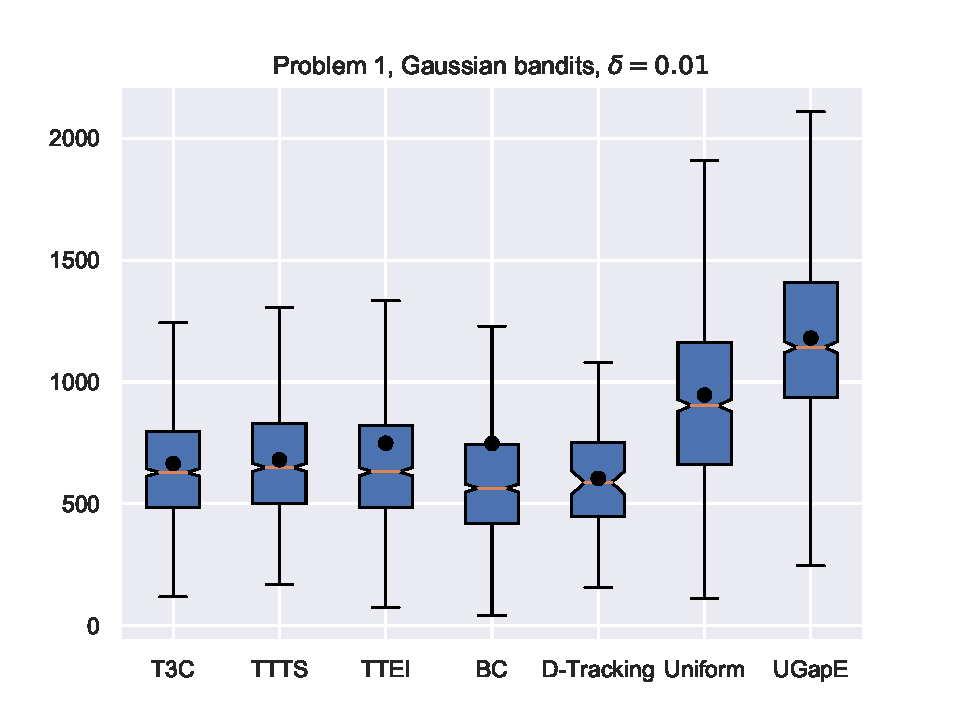
\includegraphics[clip, width= 0.24\textwidth]{Chapter3/img/gaussian1.pdf}
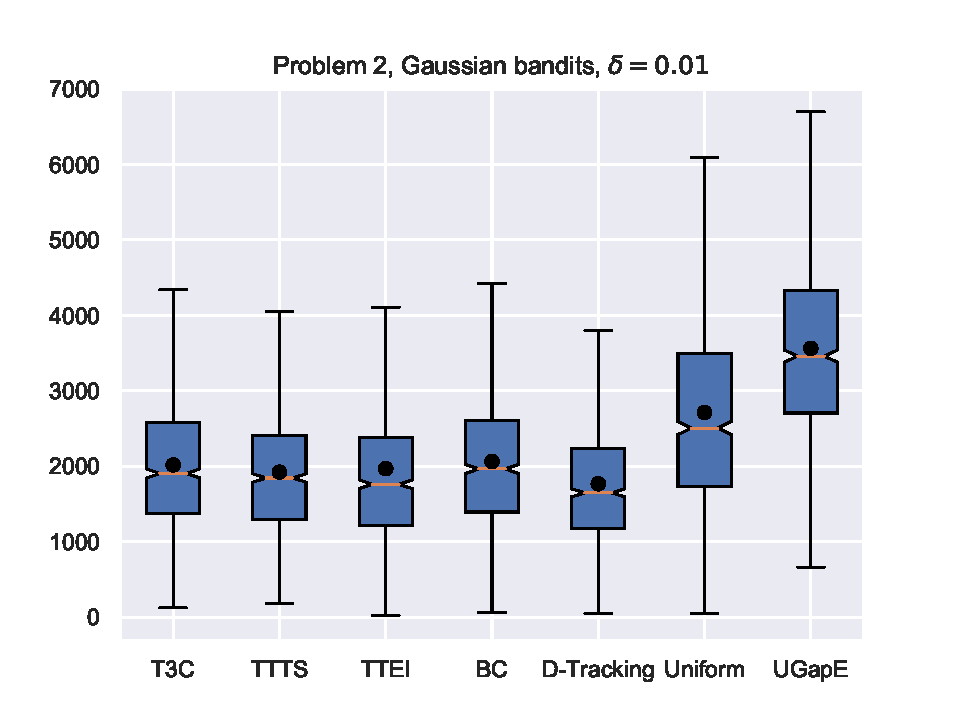
\includegraphics[clip, width= 0.24\textwidth]{Chapter3/img/gaussian2.pdf}
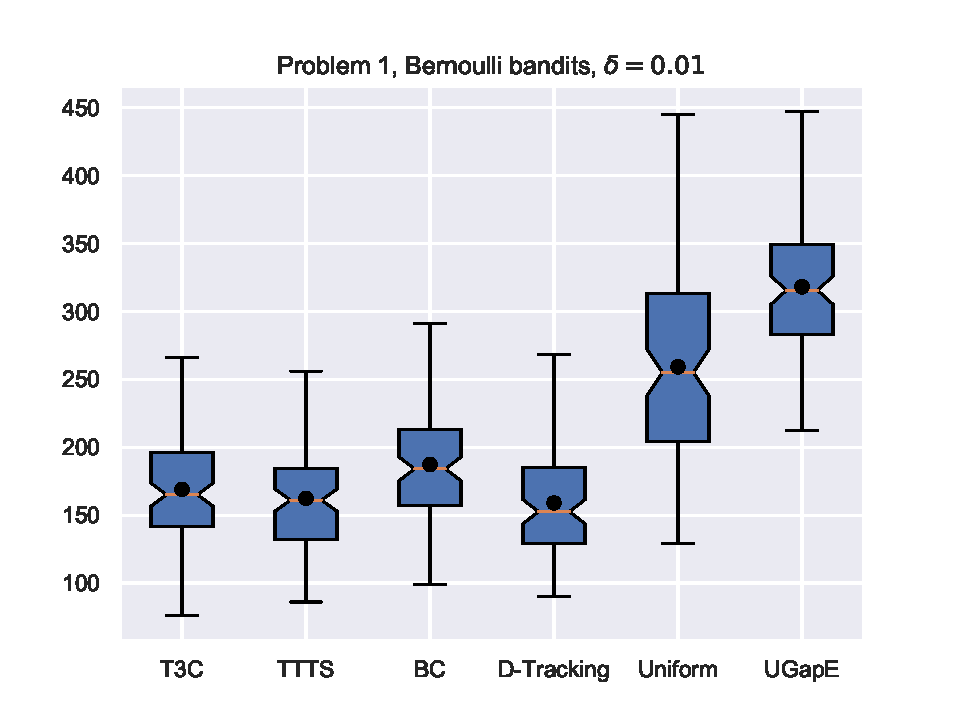
\includegraphics[clip, width= 0.24\textwidth]{Chapter3/img/bernoulli1.pdf}
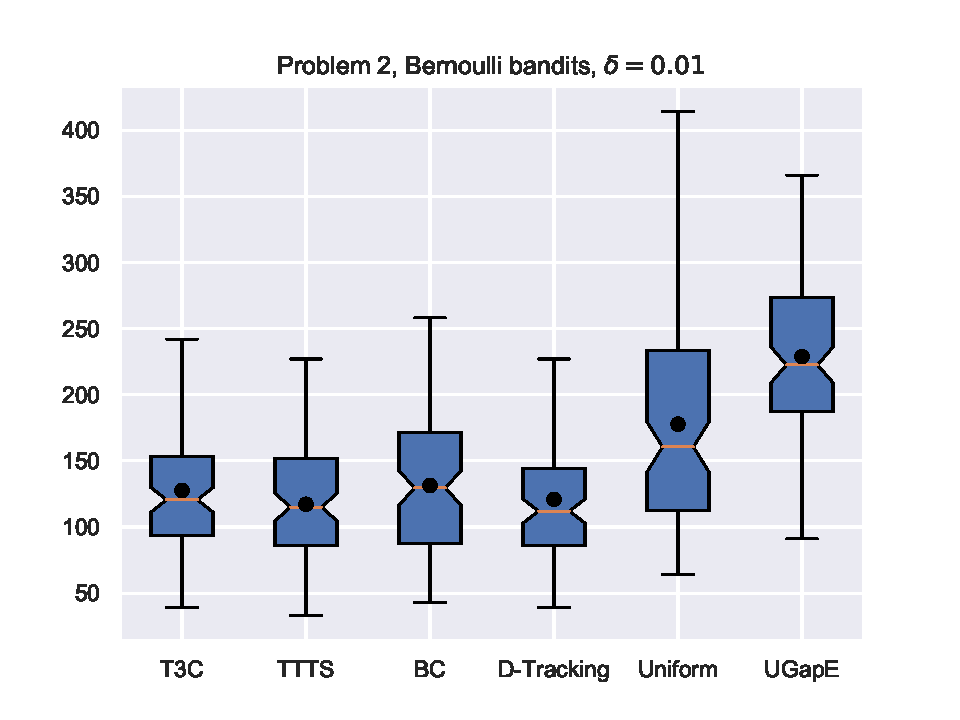
\includegraphics[clip, width= 0.24\textwidth]{Chapter3/img/bernoulli2.pdf}
\caption{Sample complexity of different BAI sampling rules over some random problem instances. Black dots represent means and oranges lines represent medians.}
\label{fig:confidence}
\end{figure*}

\begin{table*}[t!]
\centering
\small
%\def\arraystretch{1.2}
\begin{tabular}{|c|c|c|c|c|c|c|c|}
 \hline
 \textbf{Sampling rule} & \TCC & \TTTS & \TTEI & \BC & \DT & \texttt{Uniform} & \UGapE \\
 \hline
 \textbf{Execution time (s)} & $1.6\times 10^{-5}$ & $2.3\times 10^{-4}$ & $1\times 10^{-5}$ & $1.4\times 10^{-5}$ & $1.3\times 10^{-3}$ & $6\times 10^{-6}$ & $5\times 10^{-6}$ \\
 \hline
\end{tabular}
\caption{Average execution time in seconds for different BAI sampling rules.}
\label{table:time}
\end{table*}


\section{Optimal Posterior Convergence
}\label{sec:bayesian}

Recall that $a_{n, I^\star}$ denotes the posterior mass assigned to the event that action $I^\star$ (i.e.\ the true optimal arm) is optimal at time $n$. As the number of observations tends to infinity, we desire that the posterior distribution converges to the truth. In this section we show equivalently that the posterior mass on the complementory event, $1 - a_{n, I^\star}$, the event that arm $I^\star$ is not optimal, converges to zero at an exponential rate, and that it does so at optimal rate $\Gamma_{\beta}^\star$. 

\citet{russo2016ttts} proves a similar theorem under three confining boundedness assumptions (cf.\,\citealt{russo2016ttts}, Asssumption 1) on the parameter space, the prior density and the (first derivative of the) log-normalizer of the exponential family. Hence, the theorems in \cite{russo2016ttts} do not apply to the two bandit models most used in practise, which we consider in this paper: the Gaussian and Bernoulli model. 

In the first case, the parameter space is unbounded, in the latter model, the derivative of the log-normalizer (which is $e^{\eta} / (1 + e^\eta)$) is unbounded. Here we provide two theorems, proving that under \TTTS, the optimal, exponential posterior convergence rates are obtained for the Gaussian model with uninformative (improper) Gaussian priors (proof given in Appendix~\ref{app:posterior_gaussian}), and the Bernoulli model with $\cB eta(1,1)$ priors (proof given in Appendix~\ref{app:posterior_beta}).

\begin{restatable}{theorem}{restateposteriorgaussian}\label{thm:posterior_gaussian}
    Under \TTTS, for Gaussian bandits with improper Gaussian priors, it holds almost surely that 
    \[
        \lim_{n\rightarrow{\infty}} -\frac{1}{n}\log(1-a_{n,I^\star}) = \Gamma_{\beta}^\star.
    \]
\end{restatable}

\begin{restatable}{theorem}{restateposteriorbernoulli}\label{thm:posterior_bernoulli}
	Under \TTTS, for Bernoulli bandits and uniform priors, it holds almost surely that
	\[
	\lim_{n\rightarrow{\infty}} -\frac{1}{n}\log(1-a_{n,I^\star}) = \Gamma_{\beta}^\star.
	\]
\end{restatable}


%!TEX root = ../Chapter3.tex
\begin{figure*}[t!]
 \centering
 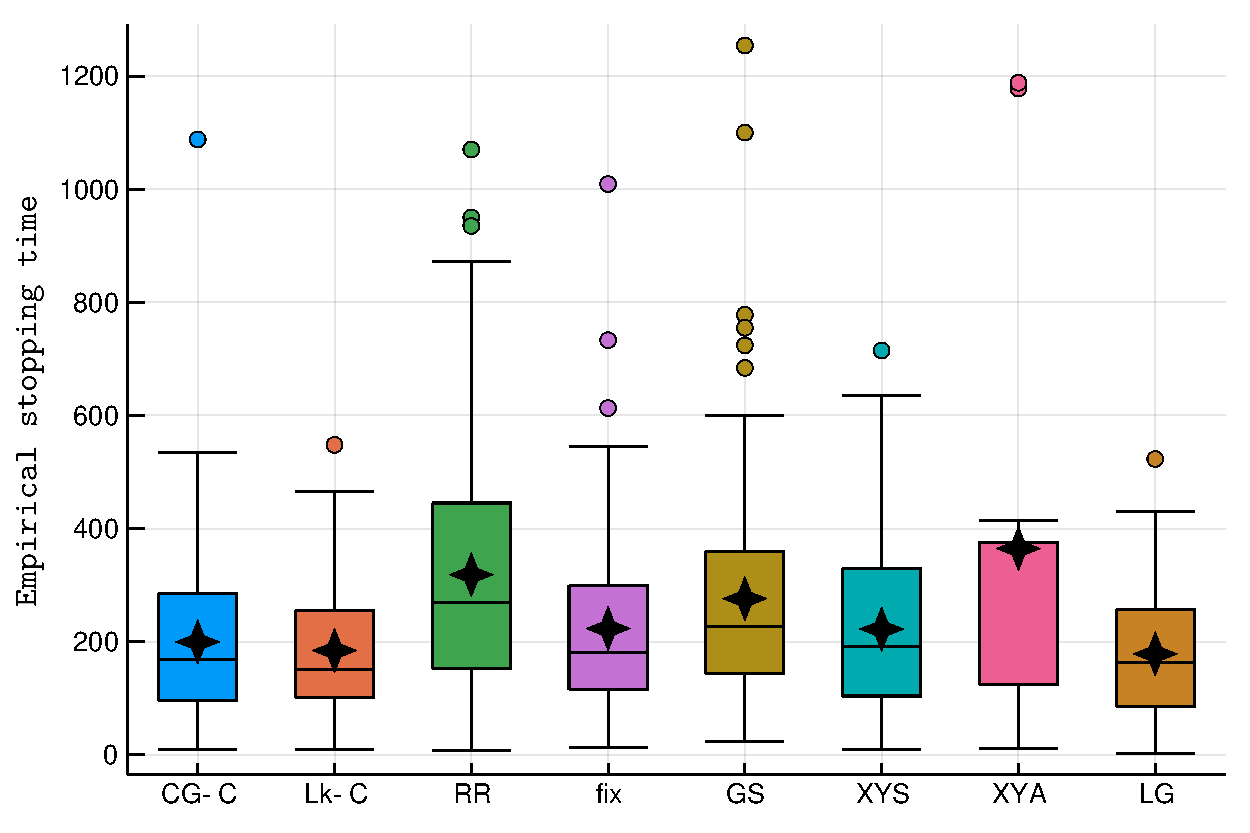
\includegraphics[clip, width= 0.3\textwidth]{Chapter3/img/bai_sin_0-1}
 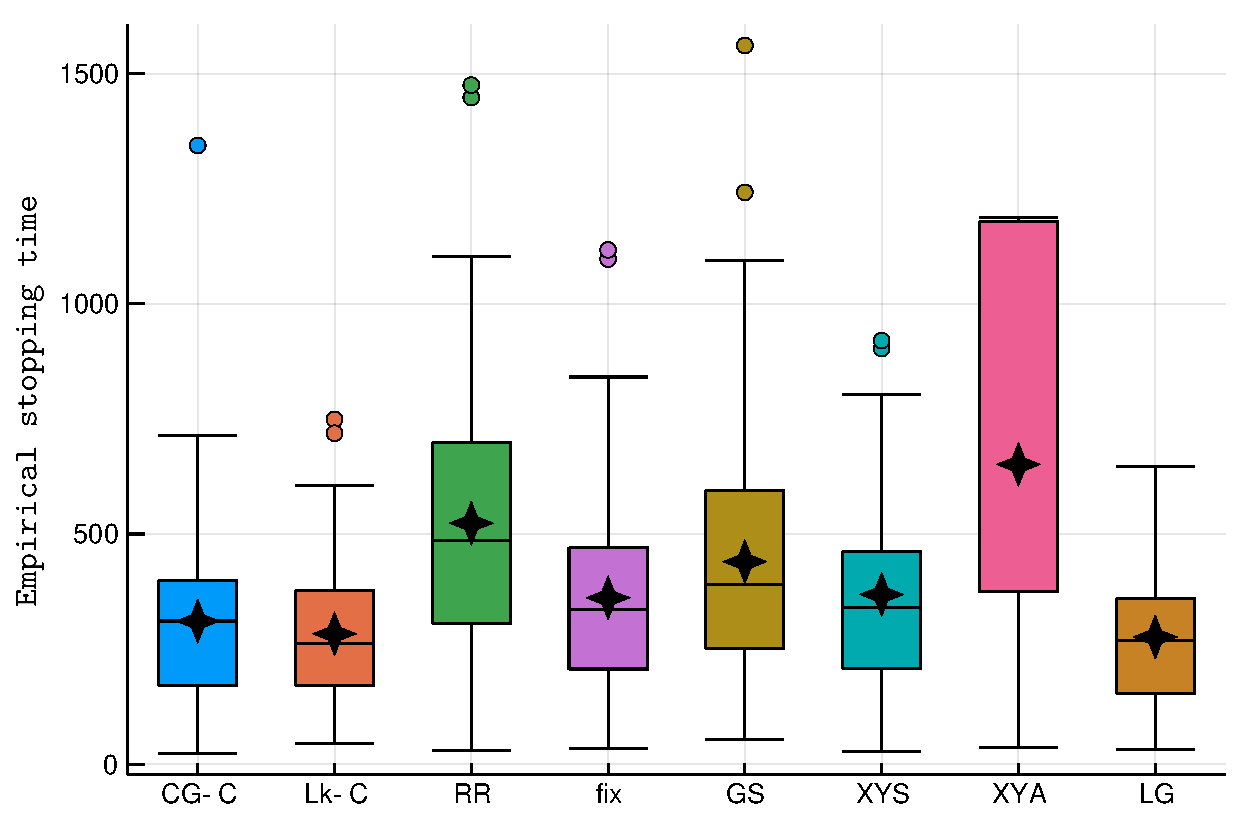
\includegraphics[clip, width= 0.3\textwidth]{Chapter3/img/bai_sin_0-01}
 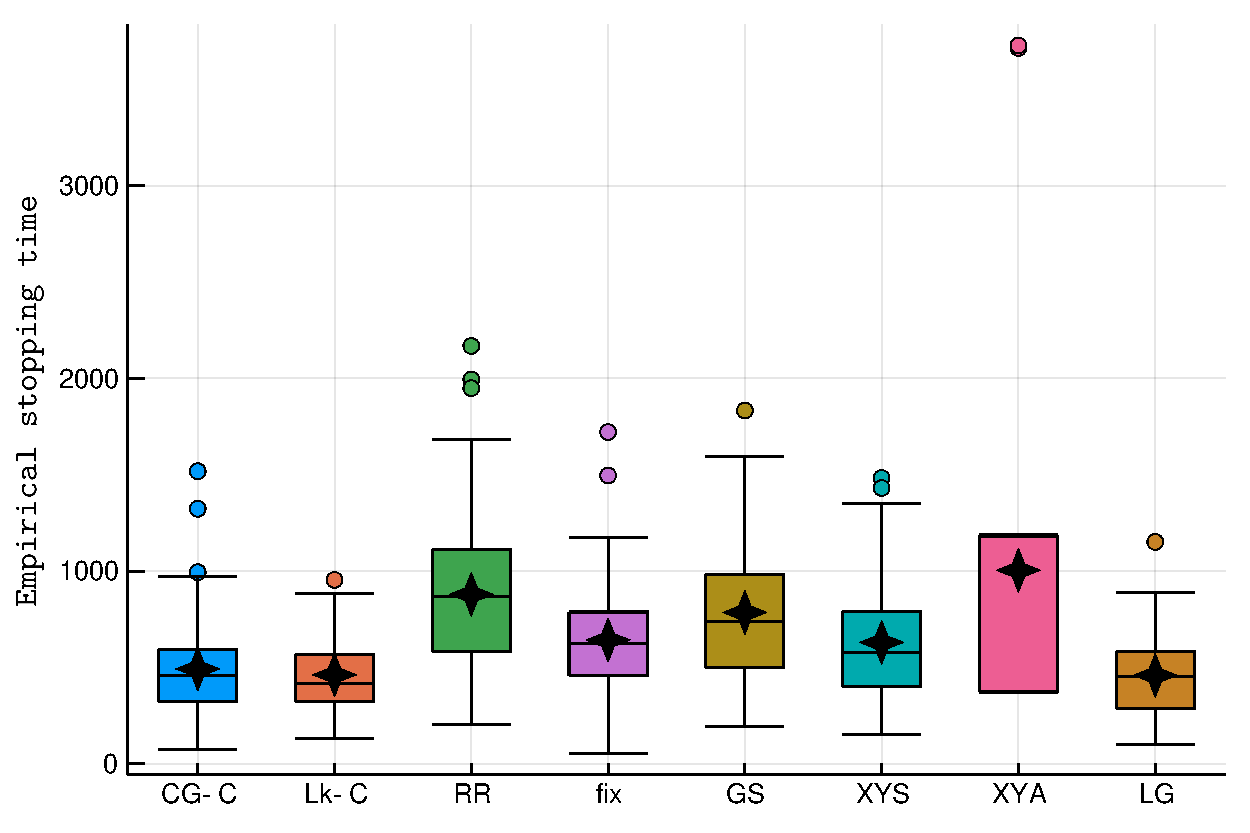
\includegraphics[clip, width= 0.3\textwidth]{Chapter3/img/bai_sin_0-0001}
 \caption{Sample complexity of different linear BAI sampling rules over the usual counter-example with $\delta=0.1, 0.01, 0.0001$ respectively. CG = \LGC,  Lk = \LG, RR = uniform sampling, fix = tracking the fixed weights, GS = \XYS with $\gopt$-allocation, XYS = \XYS with $\xyopt$-allocation, LG = \LGapE. The mean stopping time is represented by a black cross.}
 \label{fig:sample_complexity_1}
\end{figure*}

\begin{figure*}[t!]
 \centering
 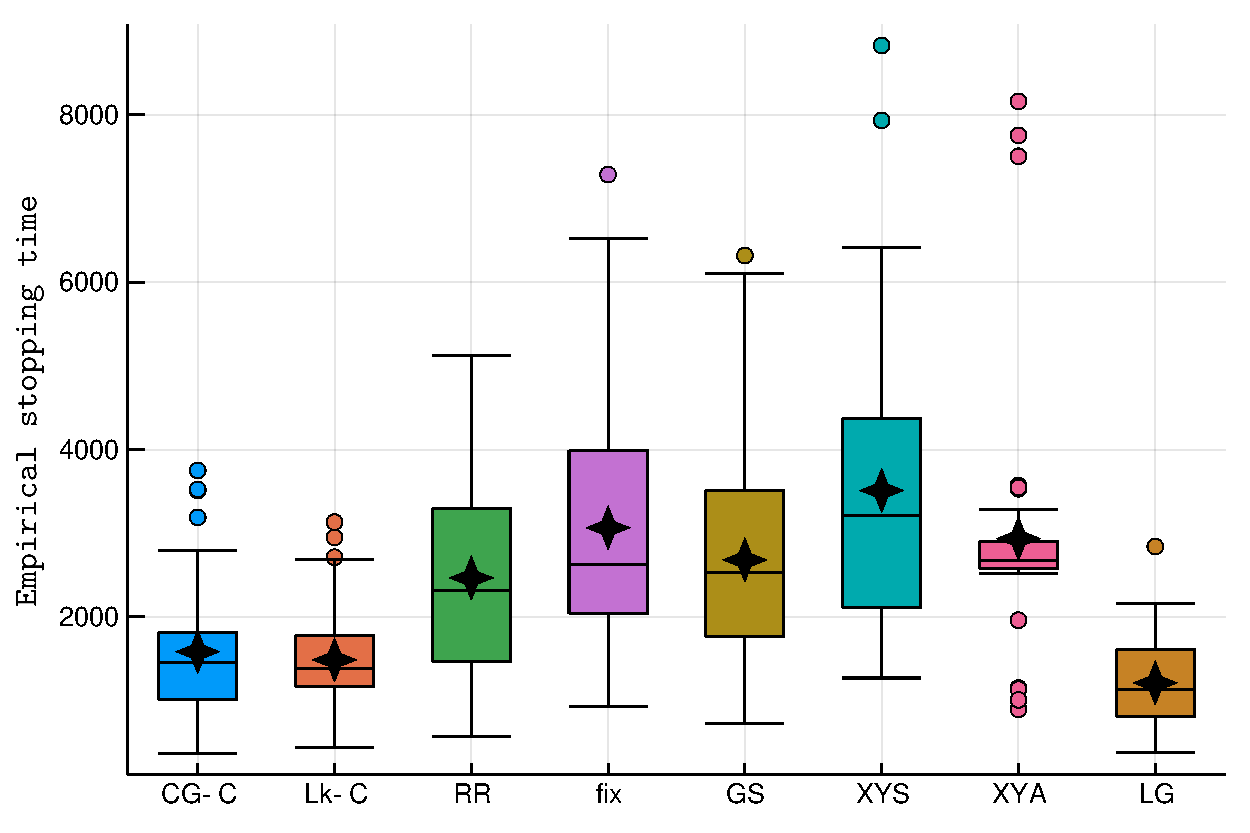
\includegraphics[clip, width= 0.24\textwidth]{Chapter3/img/bai_dim_6}
 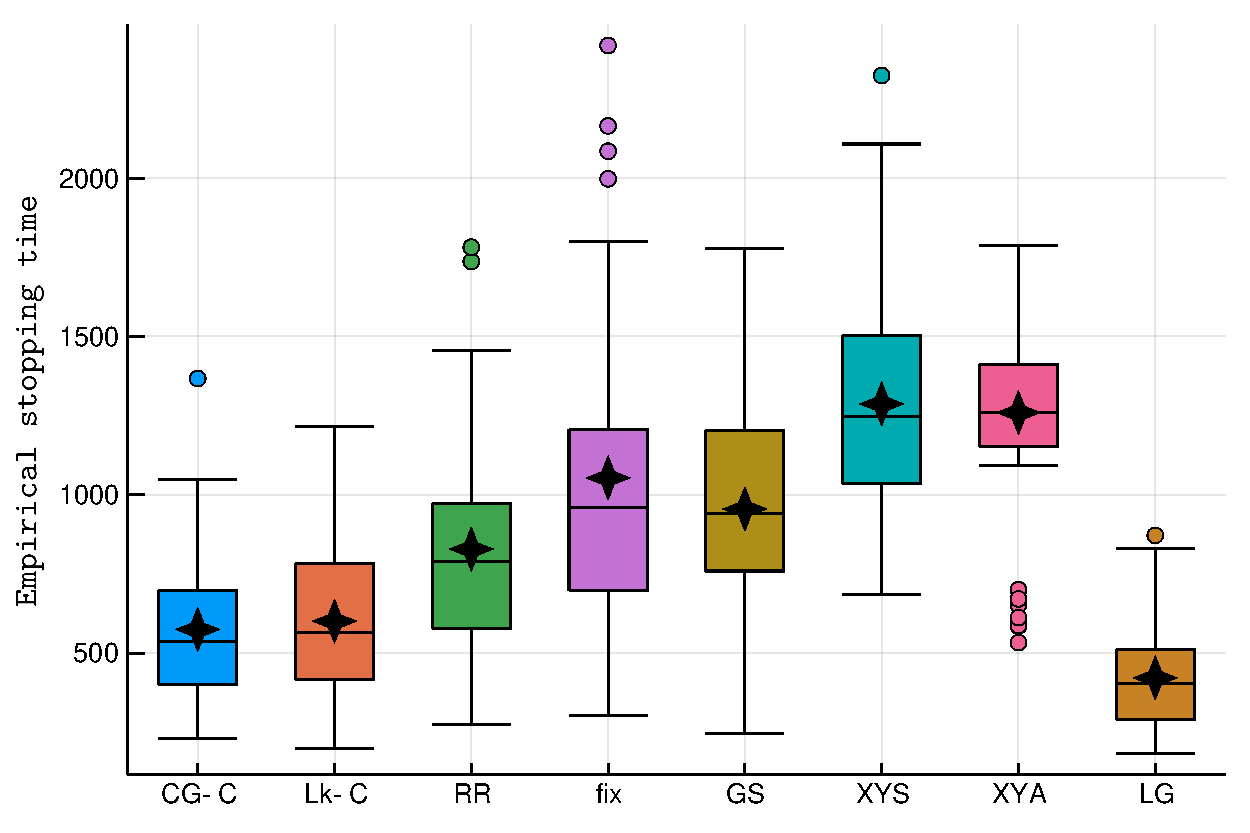
\includegraphics[clip, width= 0.24\textwidth]{Chapter3/img/bai_dim_8}
 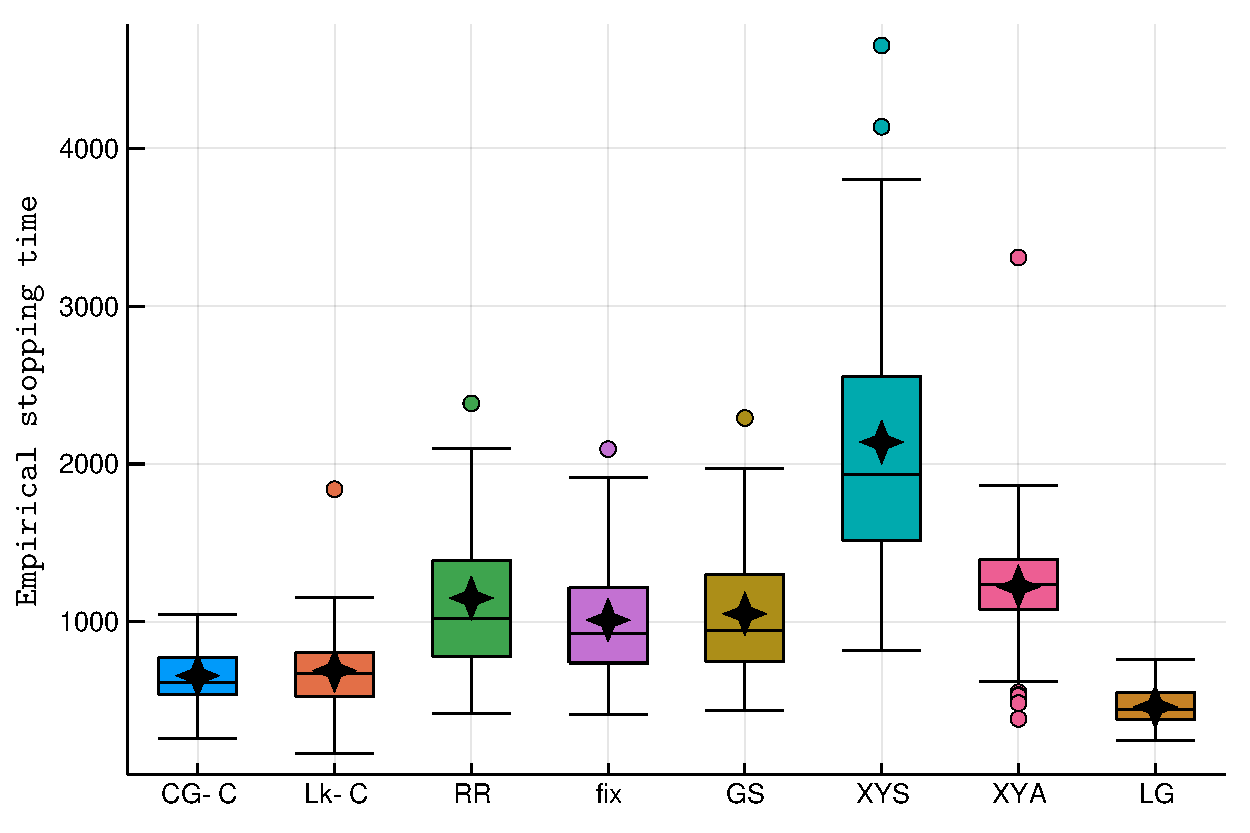
\includegraphics[clip, width= 0.24\textwidth]{Chapter3/img/bai_dim_10}
 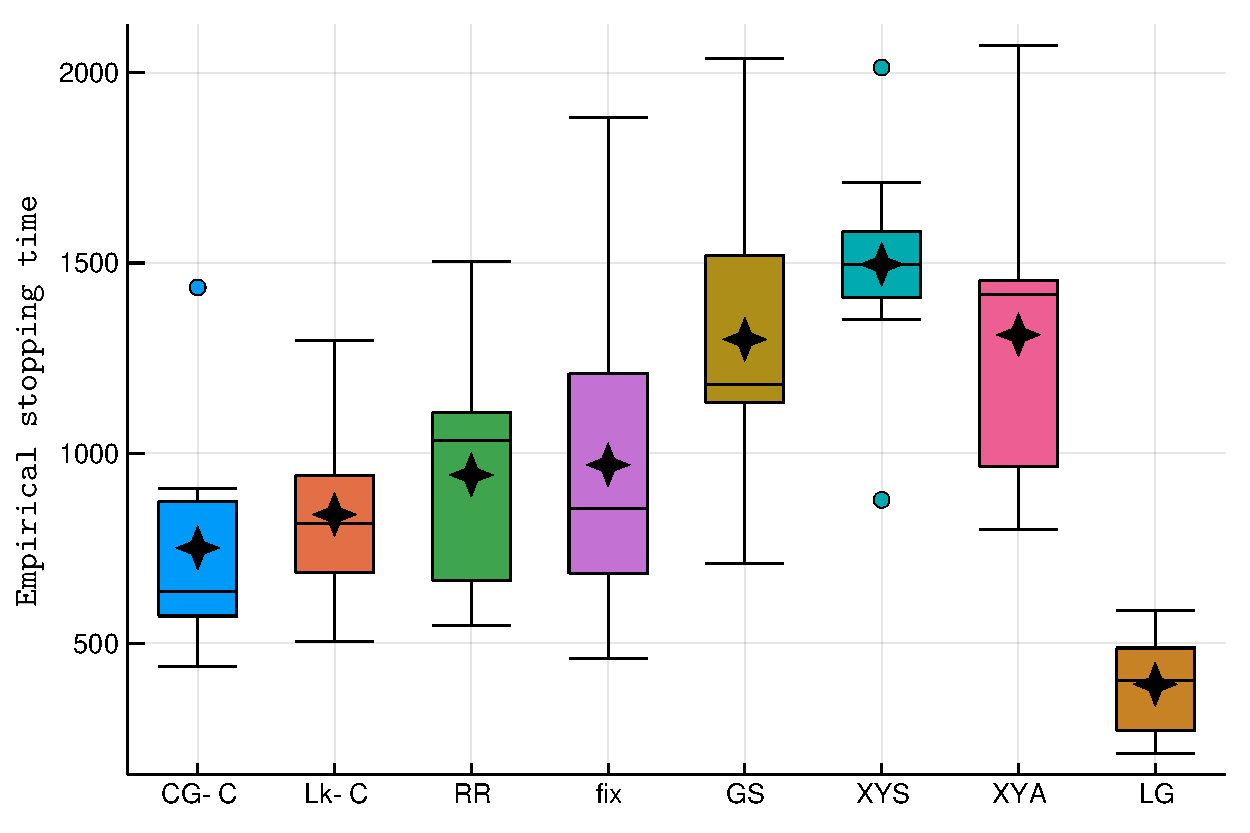
\includegraphics[clip, width= 0.24\textwidth]{Chapter3/img/bai_dim_12}
 \caption{Sample complexity of different linear BAI sampling rules over random unit sphere vectors with $d=6, 8, 10, 12$ from left to right.}
 \label{fig:sample_complexity_2}
\end{figure*}

\section{Experiments}\label{sec:lgc.experiments}
Besides our algorithms, we implement the following algorithms, all using the same stopping rule (more discussion given in Appendix~\ref{app:lgc.stopping}): uniform sampling, the greedy version of \XYS (including $\gopt$-allocation and $\xyopt$-allocation), \XYA, and the greedy version of \LGapE. We skip \GLUCB/\GLGapE since they are more or less equivalent to \LGapE in the scope of this paper.
\vspace{-0.3cm}
\paragraph{The usual hard instance.}
Usual sampling rules for classical BAI may not work for the linear case. This can be understood on a well-studied instance already discussed by~\citet{soare2014linear,xu2018linear}, which encapsulates the difficulty of BAI in a linear bandit, and thus is the first instance on which we test our algorithms. In this instance, arms are the canonical basis  $a_1 = e_1, a_2 = e_2, a_d = e_d$, plus an additional disturbing arm $a_{d+1} = (\cos(\alpha), \sin(\alpha), 0, \ldots, 0)^\top$, and a true regression parameter $\theta$ equal to $e_1$. In this problem, the best arm is always $a_1$, but when the angle $\alpha$ is small, the disturbing arm $a_{d+1}$ is hard to discriminate from $a_1$. As already argued by~\citet{soare2014linear}, an efficient sampling rule for this problem instance would rather pull $a_2$ in order to reduce the uncertainty in the direction $a_1-a_{d+1}$. Naive adaptation of classical BAI algorithms cannot deal with that situation naturally. We further use a simple set of experiments to justify that intuition. We run our two algorithms and the one of~\citet{degenne2019game} that we call \texttt{DKM} over the problem instance whence $d=2$, $\delta=0.01$ and $\alpha=0.1$. We show the number of pulls for each arm averaged over 100 replications of experiments in Table~\ref{table:pulls}. We see that, indeed, \texttt{DKM} pulls too much $a_3$, while our algorithms focus mostly on $a_2$.


\begin{table}[th]\centering
%\def\arraystretch{1.2}
\begin{tabular}{|c|c|c|c|}
 \hline
 & \LG & \LGC & \texttt{DKM} \\
 \hline
 \textbf{$a_1$} & $1912$ & $1959$ & $1943$ \\
 \hline
 \textbf{$a_2$} & $5119$ & $4818$ & $4987$ \\
 \hline
 \textbf{$a_3$} & $104$ & $77$ & $1775$ \\
 \hline
 \textbf{Total} & $7135$ & $\bf{6854}$ & $8705$ \\
 \hline
\end{tabular}
\caption{Average number of pulls of \LG and \LGC (against \texttt{DKM}) for each arm.}
\label{table:pulls}
\end{table}

\vspace{-0.3cm}
\paragraph{Comparison of different complexities.}
We use the previous setting to illustrate various complexities differ in practice. In Table~\ref{table:optimal_weights} we compare the different complexities mentioned in this paper: the characteristic time $\Tstar(\theta)$ and its associated optimal weights $\wstar_{\cA\cBstar(\theta)}$, the $\xyopt$-complexity and its associated optimal design $\wstar_{\xyopt}$, the G-optimal complexity $\gopt$ and its associated optimal design $\wstar_{\cA\cA}$. For each weight vector $w \in\{\wstar_{\cA\cBstar(\theta)},w_{\xyopt}, w_{\gopt}\}$,
 we also provide the lower bound $T_w$ given by Therorem~\ref{th:lb_genral}, i.e.
 \[
 T_w = \max_{a\neq \astar(\theta)} \frac{\big\langle \theta, \astar(\theta)-a\big\rangle^2}{2\normm{\astar(\theta)-a}_{V_w^{-1}}^2} \log(1/\delta).
\]
In particular we notice that targeting the proportions of pulls $w_{\xyopt}, w_{\gopt}$ leads to a much larger lower bound than the one obtained with the optimal weights.
\begin{table}[th]
\centering
%\def\arraystretch{1.2}
\begin{tabular}{|c|c|c|c|}
 \hline
   & $\wstar_{\cA\cBstar}$ & $\wstar_{\xyopt}$  & $\wstar_{\gopt}$   \\
 \hline
 \textbf{$a_1$} & $0.047599$ & $0.499983$ & $0.499983$ \\
 \hline
 \textbf{$a_2$} & $0.952354$ & $0.499983$ & $0.499983$ \\
 \hline
 \textbf{$a_3$} & $0.000047$ & $0.000033$ & $0.000033$ \\
 \hline
 \textbf{$T_w$} & $369$ & $2882$ & $2882$ \\
 \hline
   & $\Tstar(\theta)$ & $2\xyopt/\DeltaMin^2$ & $8\gopt/\DeltaMin^2$\\
 \hline
  \textbf{Complexity} & $0.124607$ & $32.0469$ & $64.0939$ \\
 \hline
\end{tabular}
\caption{Optimal weights for various complexities with $\DeltaMin= 0.0049958$.}
\label{table:optimal_weights}
\end{table}

\paragraph{Comparison with other algorithms.}
Finally we benchmark our two sampling rules against others from the literature. %Note that the main purpose of this paper is to propose algorithms with asymptotic optimality while being practically usable, but we do not claim to have the best performing ones.
We test over two synthetic problem instances, with the first being the previous counter-example. We set $d=2$, $\alpha=\pi/6$. Fig.~\ref{fig:sample_complexity_1} shows the empirical stopping time of each algorithms averaged over 100 runs, with a confidence level $\delta=0.1, 0.01, 0.0001$ from left to right. Our two algorithms show competitive performance (the two leftmost boxes on each plot), and are only slightly worse than \LGapE.

For the second instance, we consider 20 arms randomly generated from the unit sphere $\mathbb{S}^{d-1}\eqdef\{a\in\R^d; \normm{a}_2=1\}$. We choose the two closest arms $a, a'$ and we set $\theta = a + 0.01(a'-a)$ so that a is the best arm. This setting has already been considered by~\citet{tao2018alba}. We report the same box plots over 100 replications as before with increasing dimension in Fig.~\ref{fig:sample_complexity_2}. More precisely, we set $d=6, 8, 10, 12$ respectively, and always keep a same $\delta = 0.01$. Our algorithms consistently show strong performances compared to other algorithms apart from \LGapE. Moreover, we can see that in these random examples, \LGC works better than the non-confexified one, and is even competitive compared to \LGapE.

We stress that although the main focus of this paper is theoretical, with algorithms that are asymptotically optimal, our methods are also competitive with earlier algorithms experimentally.


%!TEX root = ../Chapter3.tex
\section{Discussion}\label{sec:t3c.discussion}

We have advocated the use of a Bayesian sampling rule for BAI. In particular, we proved that \TTTS and a computationally advantageous approach \TCC, are both $\beta$-optimal in the fixed-confidence setting, for Gaussian bandits. 
%Our analysis applies to Gaussian bandits, but could be extended to more distributions for which posterior tails bounds are available. 
We further extended the Bayesian optimality properties established by \cite{russo2016ttts} to more practical choices of models and prior distributions. 


In order to be optimal, the sampling rules studied in this paper would need to use the oracle tuning $\beta^\star =\argmax_{\beta \in [0,1]} \Gamma_\beta^\star$, which is not feasible. In future work, we will investigate an efficient online tuning of~$\beta$ to circumvent this issue. We also plan to investigate the extension of \TCC to more general pure exploration problems, as an alternative to approaches recently proposed by~\citet{menard2019lma,degenne2019game}.

Finally, it is also important to study Bayesian sampling rules in the fixed-budget setting which is more plausible in many application scenarios such as applying BAI for automated machine learning~\citep{hoffman2014bayesgap,li2017hyperband,shang2019dttts}.
\vfil


% \newpage
% \bibliographystyle{plainnat}
% \bibliography{Major}
% \newpage
